%CITATIONS: https://www.sharelatex.com/blog/2013/08/08/thesis-series-pt4.html

% Masters/Doctoral Thesis 
% LaTeX Template
% Version 2.4 (22/11/16)
% http://www.LaTeXTemplates.com

%----------------------------------------------------------------------------------------
%	PACKAGES AND OTHER DOCUMENT CONFIGURATIONS
%----------------------------------------------------------------------------------------

\documentclass[11pt, oneside, english, singlespacing, %TODO: twosided machen
%draft, % Uncomment to enable draft mode (no pictures, no links, overfull hboxes indicated)
%nolistspacing, % If the document is onehalfspacing or doublespacing, uncomment this to set spacing in lists to single
%liststotoc, % Uncomment to add the list of figures/tables/etc to the table of contents
%toctotoc, % Uncomment to add the main table of contents to the table of contents
%parskip, % Uncomment to add space between paragraphs
headsepline, % Uncomment to get a line under the header
%chapterinoneline, % Uncomment to place the chapter title next to the number on one line
%consistentlayout, % Uncomment to change the layout of the declaration, abstract and acknowledgements pages to match the default layout
]{MastersDoctoralThesis} 
\setcounter{tocdepth}{1}

\usepackage[utf8]{inputenc}
\usepackage[T1]{fontenc} 
\usepackage{palatino} %font style palatino
\usepackage{algorithm}
\usepackage{amsmath}
\usepackage{dsfont}
\usepackage{hyperref}
\usepackage{graphicx}
\usepackage[nodayofweek,level]{datetime}
\hypersetup{colorlinks=false} % hides the links in the PDF but not in printed text
%others would be: \hypersetup{...  urlcolor= .. citecolor = .. allcolor = .. hidelinks }
\usepackage{pifont,calc,xcolor}

\usepackage{tikz}
\usepackage{sequence_diagrams/pgf-umlsd}
\usepgflibrary{arrows} % for pgf-umlsd


%\usepackage[backend=bibtex,style=authoryear,natbib=true]{biblatex} 
\usepackage[backend=biber,natbib=true, minbibnames=5, maxbibnames=8]{biblatex} 
%\addbibresource{chapter2basics.bib}
\addbibresource{chapter3basics.bib}

%\bibliography{example.bib}


\usepackage[autostyle=true]{csquotes} 

%to include .1 files as metapost
\DeclareGraphicsRule{.1}{mps}{*}{}
\DeclareGraphicsRule{.2}{mps}{*}{}
\DeclareGraphicsRule{.3}{mps}{*}{}
\DeclareGraphicsRule{.4}{mps}{*}{}
\DeclareGraphicsRule{.5}{mps}{*}{}
\DeclareGraphicsRule{.6}{mps}{*}{}

%----------------------------------------------------------------------------------------
%	MARGIN SETTINGS
%----------------------------------------------------------------------------------------

\geometry{paper=a4paper, inner=2.5cm, outer=3.8cm, bindingoffset=.5cm, top=1.5cm, bottom=1.5cm, 
	%showframe, % Uncomment to show how the type block is set on the page
}

%----------------------------------------------------------------------------------------
%	TO INCLUDE THE CODE COMPARISONS IN THE APPENDIX
%----------------------------------------------------------------------------------------
\usepackage[scaled=0.72]{beramono}
\usepackage{parcolumns}
\usepackage{listings}
\usepackage{lscape}



\definecolor{verylightgray}{gray}{0.89}
\newlength\lsthorizontalpadding
\setlength\lsthorizontalpadding{3pt}
\newcommand*\lstnumberstyle{\ttfamily\scriptsize}
\newlength\lstnumbersep
\setlength\lstnumbersep{8pt}
\newlength\lstnumberwidth
\setlength\lstnumberwidth{\widthof{\lstnumberstyle00}+\lstnumbersep+\lsthorizontalpadding}

\newcommand{\leon}{the first supervisor~}

\makeatletter
\newcommand\footnoteref[1]{\protected@xdef\@thefnmark{\ref{#1}}\@footnotemark}
\makeatother
	
\lstdefinelanguage{Pseudo}{
	morekeywords={for, do, end},
	sensitive=false,
	morecomment=[l]{#},
	morestring=[b]",
}

\lstset{language=Python,
	commentstyle=\color{gray},
}

%------------- for code inline in the text-----------------------------------------------
\definecolor{evenmorelightgray}{gray}{0.95}
%\newcommand{\inlinecode}[1]{\colorbox{verylightgray}{\lstinline[basicstyle=\ttfamily\color{white}]{#1}}}
\newcommand{\inlinecode}[1]{\colorbox{evenmorelightgray}{\lstinline[basicstyle=\ttfamily\color{black}]{#1}}}

%----------------------------------------------------------------------------------------
%	TIKZ STUFF
%----------------------------------------------------------------------------------------


\usepackage{tikz}
\usetikzlibrary{arrows,positioning} 
\tikzset{
	%Define style for boxes
	punkt/.style={
		rectangle,
		rounded corners,
		draw=black, very thick,
		text width=6.5em,
		minimum height=2em,
		text centered}
}

\usetikzlibrary{shadows}

\newcommand*\keystroke[1]{%
	\raisebox{1px}{%
		\tikz[baseline=(key.base)]
		\node[%
		draw,
		fill=white,
		drop shadow={shadow xshift=0.25ex,shadow yshift=-0.25ex,fill=black,opacity=0.75},
		rectangle,
		rounded corners=2pt,
		inner sep=2pt,
		line width=0.5pt,
		font=\scriptsize\sffamily
		](key) {#1{\tiny\strut}}%  %originally #1\strut
		;
	}\hspace*{-0.37em}
}

%----------------------------------------------------------------------------------------
%	THESIS INFORMATION
%----------------------------------------------------------------------------------------


\thesistitle{Controlling Self-Driving Race Cars with Deep Neural Networks} %print with \ttitle

\supervisor{Leon Sütfeld \\ Prof. Dr. Gordon Pipa} %print with \supname
\examiner{}
\degree{Bachelor of Science} %print with \degreename
\author{Christoph Stenkamp} %print with \authorname
\addresses{}
\subject{Cognitive Science} %not currently used in the template, print with \subjectname
\keywords{} %not currently used in the template, print with \keywordnames
\university{University of Osnabrück} % Your university's name and URL, this is used in the title page and abstract, print it elsewhere with \univname
\department{department of neuroinformatics} % Your department's name and URL, this is used in the title page and abstract, print it elsewhere with \deptname
\group{\href{http://researchgroup.university.com}{Research Group Name}} % Your research group's name and URL, this is used in the title page, print it elsewhere with \groupname
\faculty{\href{http://faculty.university.com}{Faculty Name}} % Your faculty's name and URL, this is used in the title page and abstract, print it elsewhere with \facname

\AtBeginDocument{
	\hypersetup{pdftitle=\ttitle} 
	\hypersetup{pdfauthor=\authorname} 
	\hypersetup{pdfkeywords=\keywordnames} 
}


\begin{document}
	
	\frontmatter % Use roman page numbering style (i, ii, iii, iv...) for the pre-content pages
	
	\pagestyle{plain} % Default to the plain heading style until the thesis style is called for the body content
	

%----------------------------------------------------------------------------------------
%	TITLE PAGE
%----------------------------------------------------------------------------------------

	\begin{titlepage}
		\begin{center}
			
			\includegraphics[scale = 0.7]{Logo} % University/department logo - uncomment to place it
			
			\vspace*{.06\textheight}
			\HRule \\[0.4cm] % Horizontal line
			{\huge \bfseries \ttitle\par}\vspace{0.4cm} % Thesis title
			\HRule \\[1.5cm] % Horizontal line
			
			%\vspace*{.06\textheight}
			{\scshape\LARGE \univname\par}\vspace{.5cm} % University name
			
			{\scshape\Large \deptname \par}\vspace{1.5cm}
			
			\textsc{\Large Bachelor's Thesis}\\[0.5cm] % Thesis type
			
			\vspace*{.1\textheight} 
			\begin{minipage}[t]{0.4\textwidth}
				\begin{flushleft} \large
					\emph{Author:}\\
					\authorname % Author name - remove the \href bracket to remove the link
				\end{flushleft}
			\end{minipage}
			\begin{minipage}[t]{0.4\textwidth}
				\begin{flushright} \large
					\emph{Supervisors:} \\
					\supname % Supervisor name - remove the \href bracket to remove the link  
				\end{flushright}
			\end{minipage}\\[3cm]

			\vfill
			Osnabrück,\\
			\today
			
		\end{center}
	\end{titlepage}	

	%----------------------------------------------------------------------------------------
	%	ABSTRACT PAGE
	%----------------------------------------------------------------------------------------
	
	\begin{abstract}
		\addchaptertocentry{\abstractname} % Add the abstract to the table of contents
		This Thesis will be written in the next two months, and I'm pretty scared about that.\\
		TODO: sobald der komplette text steht bei den Formeln auf die nicht referenziert wird die nummern weg machen (equation*)
	\end{abstract}

	%----------------------------------------------------------------------------------------
	%	PREFACE PAGE
	%----------------------------------------------------------------------------------------

	\begin{preface}{\authorname}{Osnabrück, \today}
		\addchaptertocentry{\prefacename}
		\noindent This document was written as the author’s bachelor thesis at the \deptname~at the \univname~during summer 2017 and is an original and independent work by the author \authorname.
	\end{preface}



	
	%----------------------------------------------------------------------------------------
	%	ACKNOWLEDGEMENTS
	%----------------------------------------------------------------------------------------
	
	\begin{acknowledgements}
		\addchaptertocentry{\acknowledgementname} % Add the acknowledgements to the table of contents
		Thanks to my parents, Marie, my supervisors, and my friends.\ldots
	\end{acknowledgements}
	
	
	%----------------------------------------------------------------------------------------
	%	QUOTATION PAGE
	%----------------------------------------------------------------------------------------
	
	\newpage
	\vspace*{0.2\textheight}
	
	\noindent\enquote{\itshape There are no surprising facts, only models that are surprised by facts; and if a model is surprised by the facts, it is no credit to that model.}\bigbreak
	
	\hfill Eliezer Yudkowsky


	%----------------------------------------------------------------------------------------
	%	LIST OF CONTENTS/FIGURES/TABLES PAGES
	%----------------------------------------------------------------------------------------
	
	\tableofcontents % Prints the main table of contents
%	\addchaptertocentry{Table of Contents} %TODO: das ist die falsche seite!!!
	
	\listoffigures % Prints the list of figures
%	\addchaptertocentry{List of Figures}
	
	\listoftables % Prints the list of tables
%	\addchaptertocentry{List of Tables}
	
	\listofalgorithms
%	\addchaptertocentry{List of Algorithms}
	%https://tex.stackexchange.com/questions/100346/typesetting-listofalgorithms-like-listoffigures-and-listoftables-using-titletoc
	%http://latex.org/forum/viewtopic.php?f=59&t=26383
	
	%----------------------------------------------------------------------------------------
	%	ABBREVIATIONS
	%----------------------------------------------------------------------------------------
	\newcommand{\abbrevtext}{The abbreviations used throughout the work are compiled in the following list below. Note that the abbreviations denote the singular form of the abbreviated words. Whenever the plural forms is needed, an s is added. Thus, for example, whereas ANN abbreviates \textit{artificial neural network}, the abbreviation of\textit{ artificial neural networks} is written ANNs.}

	\begin{abbreviations}{ll}[\abbrevtext] % Include a list of abbreviations (a table of two columns)
		
%		\addchaptertocentry{\abbrevname}
		\textbf{ANN}	& \textbf{A}rtificial \textbf{N}eural \textbf{N}etwork\\
		\textbf{API}	& \textbf{A}pplication \textbf{P}rogramming \textbf{I}nterface\\
		\textbf{CNN} 	& \textbf{C}onvolutional (artificial) \textbf{N}eural \textbf{N}etwork\\
		\textbf{CPU} 	& \textbf{C}entral \textbf{P}rocessing \textbf{U}nit\\
		\textbf{DDPG} 	& \textbf{D}eep \textbf{D}eterministic \textbf{P}olicy \textbf{G}radient - Network\\
		\textbf{DQN} 	& \textbf{D}eep-\textbf{Q}-\textbf{N}etwork\\
		\textbf{FPS} 	& \textbf{F}rames \textbf{P}er \textbf{S}econd\\
		\textbf{GUI} 	& \textbf{G}raphical \textbf{U}ser \textbf{I}nterface\\
		\textbf{MDP}	& \textbf{M}arkov \textbf{D}ecision \textbf{P}rocess\\
		\textbf{POMDP} 	& \textbf{P}artially \textbf{O}bserved \textbf{M}arkov \textbf{D}ecision \textbf{P}rocess\\
		
	\end{abbreviations}
	
	%----------------------------------------------------------------------------------------
	%	SYMBOLS
	%----------------------------------------------------------------------------------------
	
	\begin{symbols}{lll} % Include a list of Symbols (a three column table)
		
%		\addchaptertocentry{\symbolsname}
		%TODO: die hier schöner, mit text drüber a la einheitliche symbole etc, und spaltennamen!
		
%		$a$ & distance & \si{\meter} \\
%		$P$ & power & \si{\watt} (\si{\joule\per\second}) \\
%		%Symbol & Name & Unit \\
%		
%		\addlinespace % Gap to separate the Roman symbols from the Greek (innerhalb derer: ALPHABETISCH)
%		
%		$\omega$ & angular frequency & \si{\radian} \\
		
	\end{symbols}
	
	%----------------------------------------------------------------------------------------
	%	DEDICATION
	%----------------------------------------------------------------------------------------
	
	\dedicatory{For my friends, family, and especially Marie.} 
	
	%----------------------------------------------------------------------------------------
	%	THESIS CONTENT - CHAPTERS
	%----------------------------------------------------------------------------------------
	
	\mainmatter % Begin numeric (1,2,3...) page numbering
	
	\pagestyle{thesis} % Return the page headers back to the "thesis" style
	
	% Include the chapters of the thesis as separate files from the Chapters folder
	% Uncomment the lines as you write the chapters
	
	% Chapter 1

\chapter{Chapter Title Here} % Main chapter title

\label{Chapter1} % For referencing the chapter elsewhere, use \ref{Chapter1} 

%----------------------------------------------------------------------------------------

% Define some commands to keep the formatting separated from the content 
\newcommand{\keyword}[1]{\textbf{#1}}
\newcommand{\tabhead}[1]{\textbf{#1}}
\newcommand{\code}[1]{\texttt{#1}}
\newcommand{\file}[1]{\texttt{\bfseries#1}}
\newcommand{\option}[1]{\texttt{\itshape#1}}

%----------------------------------------------------------------------------------------

\section{Welcome and Thank You}
Welcome to this \LaTeX{} Thesis Template, a beautiful and easy to use template for writing a thesis using the \LaTeX{} typesetting system.

If you are writing a thesis (or will be in the future) and its subject is technical or mathematical (though it doesn't have to be), then creating it in \LaTeX{} is highly recommended as a way to make sure you can just get down to the essential writing without having to worry over formatting or wasting time arguing with your word processor.

\LaTeX{} is easily able to professionally typeset documents that run to hundreds or thousands of pages long. With simple mark-up commands, it automatically sets out the table of contents, margins, page headers and footers and keeps the formatting consistent and beautiful. One of its main strengths is the way it can easily typeset mathematics, even \emph{heavy} mathematics. Even if those equations are the most horribly twisted and most difficult mathematical problems that can only be solved on a super-computer, you can at least count on \LaTeX{} to make them look stunning.

%----------------------------------------------------------------------------------------

\section{Learning \LaTeX{}}

\LaTeX{} is not a \textsc{wysiwyg} (What You See is What You Get) program, unlike word processors such as Microsoft Word or Apple's Pages. Instead, a document written for \LaTeX{} is actually a simple, plain text file that contains \emph{no formatting}. You tell \LaTeX{} how you want the formatting in the finished document by writing in simple commands amongst the text, for example, if I want to use \emph{italic text for emphasis}, I write the \verb|\emph{text}| command and put the text I want in italics in between the curly braces. This means that \LaTeX{} is a \enquote{mark-up} language, very much like HTML.

\subsection{A (not so short) Introduction to \LaTeX{}}

If you are new to \LaTeX{}, there is a very good eBook -- freely available online as a PDF file -- called, \enquote{The Not So Short Introduction to \LaTeX{}}. The book's title is typically shortened to just \emph{lshort}. You can download the latest version (as it is occasionally updated) from here:
\url{http://www.ctan.org/tex-archive/info/lshort/english/lshort.pdf}

It is also available in several other languages. Find yours from the list on this page: \url{http://www.ctan.org/tex-archive/info/lshort/}

It is recommended to take a little time out to learn how to use \LaTeX{} by creating several, small `test' documents, or having a close look at several templates on:\\ 
\url{http://www.LaTeXTemplates.com}\\ 
Making the effort now means you're not stuck learning the system when what you \emph{really} need to be doing is writing your thesis.

\subsection{A Short Math Guide for \LaTeX{}}

If you are writing a technical or mathematical thesis, then you may want to read the document by the AMS (American Mathematical Society) called, \enquote{A Short Math Guide for \LaTeX{}}. It can be found online here:
\url{http://www.ams.org/tex/amslatex.html}
under the \enquote{Additional Documentation} section towards the bottom of the page.

\subsection{Common \LaTeX{} Math Symbols}
There are a multitude of mathematical symbols available for \LaTeX{} and it would take a great effort to learn the commands for them all. The most common ones you are likely to use are shown on this page:
\url{http://www.sunilpatel.co.uk/latex-type/latex-math-symbols/}

You can use this page as a reference or crib sheet, the symbols are rendered as large, high quality images so you can quickly find the \LaTeX{} command for the symbol you need.

\subsection{\LaTeX{} on a Mac}
 
The \LaTeX{} distribution is available for many systems including Windows, Linux and Mac OS X. The package for OS X is called MacTeX and it contains all the applications you need -- bundled together and pre-customized -- for a fully working \LaTeX{} environment and work flow.
 
MacTeX includes a custom dedicated \LaTeX{} editor called TeXShop for writing your `\file{.tex}' files and BibDesk: a program to manage your references and create your bibliography section just as easily as managing songs and creating playlists in iTunes.

%----------------------------------------------------------------------------------------

\section{Getting Started with this Template}

If you are familiar with \LaTeX{}, then you should explore the directory structure of the template and then proceed to place your own information into the \emph{THESIS INFORMATION} block of the \file{main.tex} file. You can then modify the rest of this file to your unique specifications based on your degree/university. Section \ref{FillingFile} on page \pageref{FillingFile} will help you do this. Make sure you also read section \ref{ThesisConventions} about thesis conventions to get the most out of this template.

If you are new to \LaTeX{} it is recommended that you carry on reading through the rest of the information in this document.

Before you begin using this template you should ensure that its style complies with the thesis style guidelines imposed by your institution. In most cases this template style and layout will be suitable. If it is not, it may only require a small change to bring the template in line with your institution's recommendations. These modifications will need to be done on the \file{MastersDoctoralThesis.cls} file.

\subsection{About this Template}

This \LaTeX{} Thesis Template is originally based and created around a \LaTeX{} style file created by Steve R.\ Gunn from the University of Southampton (UK), department of Electronics and Computer Science. You can find his original thesis style file at his site, here:
\url{http://www.ecs.soton.ac.uk/~srg/softwaretools/document/templates/}

Steve's \file{ecsthesis.cls} was then taken by Sunil Patel who modified it by creating a skeleton framework and folder structure to place the thesis files in. The resulting template can be found on Sunil's site here:
\url{http://www.sunilpatel.co.uk/thesis-template}

Sunil's template was made available through \url{http://www.LaTeXTemplates.com} where it was modified many times based on user requests and questions. Version 2.0 and onwards of this template represents a major modification to Sunil's template and is, in fact, hardly recognisable. The work to make version 2.0 possible was carried out by \href{mailto:vel@latextemplates.com}{Vel} and Johannes Böttcher.

%----------------------------------------------------------------------------------------

\section{What this Template Includes}

\subsection{Folders}

This template comes as a single zip file that expands out to several files and folders. The folder names are mostly self-explanatory:

\keyword{Appendices} -- this is the folder where you put the appendices. Each appendix should go into its own separate \file{.tex} file. An example and template are included in the directory.

\keyword{Chapters} -- this is the folder where you put the thesis chapters. A thesis usually has about six chapters, though there is no hard rule on this. Each chapter should go in its own separate \file{.tex} file and they can be split as:
\begin{itemize}
\item Chapter 1: Introduction to the thesis topic
\item Chapter 2: Background information and theory
\item Chapter 3: (Laboratory) experimental setup
\item Chapter 4: Details of experiment 1
\item Chapter 5: Details of experiment 2
\item Chapter 6: Discussion of the experimental results
\item Chapter 7: Conclusion and future directions
\end{itemize}
This chapter layout is specialised for the experimental sciences, your discipline may be different.

\keyword{Figures} -- this folder contains all figures for the thesis. These are the final images that will go into the thesis document.

\subsection{Files}

Included are also several files, most of them are plain text and you can see their contents in a text editor. After initial compilation, you will see that more auxiliary files are created by \LaTeX{} or BibTeX and which you don't need to delete or worry about:

\keyword{example.bib} -- this is an important file that contains all the bibliographic information and references that you will be citing in the thesis for use with BibTeX. You can write it manually, but there are reference manager programs available that will create and manage it for you. Bibliographies in \LaTeX{} are a large subject and you may need to read about BibTeX before starting with this. Many modern reference managers will allow you to export your references in BibTeX format which greatly eases the amount of work you have to do.

\keyword{MastersDoctoralThesis.cls} -- this is an important file. It is the class file that tells \LaTeX{} how to format the thesis. 

\keyword{main.pdf} -- this is your beautifully typeset thesis (in the PDF file format) created by \LaTeX{}. It is supplied in the PDF with the template and after you compile the template you should get an identical version.

\keyword{main.tex} -- this is an important file. This is the file that you tell \LaTeX{} to compile to produce your thesis as a PDF file. It contains the framework and constructs that tell \LaTeX{} how to layout the thesis. It is heavily commented so you can read exactly what each line of code does and why it is there. After you put your own information into the \emph{THESIS INFORMATION} block -- you have now started your thesis!

Files that are \emph{not} included, but are created by \LaTeX{} as auxiliary files include:

\keyword{main.aux} -- this is an auxiliary file generated by \LaTeX{}, if it is deleted \LaTeX{} simply regenerates it when you run the main \file{.tex} file.

\keyword{main.bbl} -- this is an auxiliary file generated by BibTeX, if it is deleted, BibTeX simply regenerates it when you run the \file{main.aux} file. Whereas the \file{.bib} file contains all the references you have, this \file{.bbl} file contains the references you have actually cited in the thesis and is used to build the bibliography section of the thesis.

\keyword{main.blg} -- this is an auxiliary file generated by BibTeX, if it is deleted BibTeX simply regenerates it when you run the main \file{.aux} file.

\keyword{main.lof} -- this is an auxiliary file generated by \LaTeX{}, if it is deleted \LaTeX{} simply regenerates it when you run the main \file{.tex} file. It tells \LaTeX{} how to build the \emph{List of Figures} section.

\keyword{main.log} -- this is an auxiliary file generated by \LaTeX{}, if it is deleted \LaTeX{} simply regenerates it when you run the main \file{.tex} file. It contains messages from \LaTeX{}, if you receive errors and warnings from \LaTeX{}, they will be in this \file{.log} file.

\keyword{main.lot} -- this is an auxiliary file generated by \LaTeX{}, if it is deleted \LaTeX{} simply regenerates it when you run the main \file{.tex} file. It tells \LaTeX{} how to build the \emph{List of Tables} section.

\keyword{main.out} -- this is an auxiliary file generated by \LaTeX{}, if it is deleted \LaTeX{} simply regenerates it when you run the main \file{.tex} file.

So from this long list, only the files with the \file{.bib}, \file{.cls} and \file{.tex} extensions are the most important ones. The other auxiliary files can be ignored or deleted as \LaTeX{} and BibTeX will regenerate them.

%----------------------------------------------------------------------------------------

\section{Filling in Your Information in the \file{main.tex} File}\label{FillingFile}

You will need to personalise the thesis template and make it your own by filling in your own information. This is done by editing the \file{main.tex} file in a text editor or your favourite LaTeX environment.

Open the file and scroll down to the third large block titled \emph{THESIS INFORMATION} where you can see the entries for \emph{University Name}, \emph{Department Name}, etc \ldots

Fill out the information about yourself, your group and institution. You can also insert web links, if you do, make sure you use the full URL, including the \code{http://} for this. If you don't want these to be linked, simply remove the \verb|\href{url}{name}| and only leave the name.

When you have done this, save the file and recompile \code{main.tex}. All the information you filled in should now be in the PDF, complete with web links. You can now begin your thesis proper!

%----------------------------------------------------------------------------------------

\section{The \code{main.tex} File Explained}

The \file{main.tex} file contains the structure of the thesis. There are plenty of written comments that explain what pages, sections and formatting the \LaTeX{} code is creating. Each major document element is divided into commented blocks with titles in all capitals to make it obvious what the following bit of code is doing. Initially there seems to be a lot of \LaTeX{} code, but this is all formatting, and it has all been taken care of so you don't have to do it.

Begin by checking that your information on the title page is correct. For the thesis declaration, your institution may insist on something different than the text given. If this is the case, just replace what you see with what is required in the \emph{DECLARATION PAGE} block.

Then comes a page which contains a funny quote. You can put your own, or quote your favourite scientist, author, person, and so on. Make sure to put the name of the person who you took the quote from.

Following this is the abstract page which summarises your work in a condensed way and can almost be used as a standalone document to describe what you have done. The text you write will cause the heading to move up so don't worry about running out of space.

Next come the acknowledgements. On this page, write about all the people who you wish to thank (not forgetting parents, partners and your advisor/supervisor).

The contents pages, list of figures and tables are all taken care of for you and do not need to be manually created or edited. The next set of pages are more likely to be optional and can be deleted since they are for a more technical thesis: insert a list of abbreviations you have used in the thesis, then a list of the physical constants and numbers you refer to and finally, a list of mathematical symbols used in any formulae. Making the effort to fill these tables means the reader has a one-stop place to refer to instead of searching the internet and references to try and find out what you meant by certain abbreviations or symbols.

The list of symbols is split into the Roman and Greek alphabets. Whereas the abbreviations and symbols ought to be listed in alphabetical order (and this is \emph{not} done automatically for you) the list of physical constants should be grouped into similar themes.

The next page contains a one line dedication. Who will you dedicate your thesis to?

Finally, there is the block where the chapters are included. Uncomment the lines (delete the \code{\%} character) as you write the chapters. Each chapter should be written in its own file and put into the \emph{Chapters} folder and named \file{Chapter1}, \file{Chapter2}, etc\ldots Similarly for the appendices, uncomment the lines as you need them. Each appendix should go into its own file and placed in the \emph{Appendices} folder.

After the preamble, chapters and appendices finally comes the bibliography. The bibliography style (called \option{authoryear}) is used for the bibliography and is a fully featured style that will even include links to where the referenced paper can be found online. Do not underestimate how grateful your reader will be to find that a reference to a paper is just a click away. Of course, this relies on you putting the URL information into the BibTeX file in the first place.

%----------------------------------------------------------------------------------------

\section{Thesis Features and Conventions}\label{ThesisConventions}

To get the best out of this template, there are a few conventions that you may want to follow.

One of the most important (and most difficult) things to keep track of in such a long document as a thesis is consistency. Using certain conventions and ways of doing things (such as using a Todo list) makes the job easier. Of course, all of these are optional and you can adopt your own method.

\subsection{Printing Format}

This thesis template is designed for double sided printing (i.e. content on the front and back of pages) as most theses are printed and bound this way. Switching to one sided printing is as simple as uncommenting the \option{oneside} option of the \code{documentclass} command at the top of the \file{main.tex} file. You may then wish to adjust the margins to suit specifications from your institution.

The headers for the pages contain the page number on the outer side (so it is easy to flick through to the page you want) and the chapter name on the inner side.

The text is set to 11 point by default with single line spacing, again, you can tune the text size and spacing should you want or need to using the options at the very start of \file{main.tex}. The spacing can be changed similarly by replacing the \option{singlespacing} with \option{onehalfspacing} or \option{doublespacing}.

\subsection{Using US Letter Paper}

The paper size used in the template is A4, which is the standard size in Europe. If you are using this thesis template elsewhere and particularly in the United States, then you may have to change the A4 paper size to the US Letter size. This can be done in the margins settings section in \file{main.tex}.

Due to the differences in the paper size, the resulting margins may be different to what you like or require (as it is common for institutions to dictate certain margin sizes). If this is the case, then the margin sizes can be tweaked by modifying the values in the same block as where you set the paper size. Now your document should be set up for US Letter paper size with suitable margins.

\subsection{References}

The \code{biblatex} package is used to format the bibliography and inserts references such as this one \parencite{Reference1}. The options used in the \file{main.tex} file mean that the in-text citations of references are formatted with the author(s) listed with the date of the publication. Multiple references are separated by semicolons (e.g. \parencite{Reference2, Reference1}) and references with more than three authors only show the first author with \emph{et al.} indicating there are more authors (e.g. \parencite{Reference3}). This is done automatically for you. To see how you use references, have a look at the \file{Chapter1.tex} source file. Many reference managers allow you to simply drag the reference into the document as you type.

Scientific references should come \emph{before} the punctuation mark if there is one (such as a comma or period). The same goes for footnotes\footnote{Such as this footnote, here down at the bottom of the page.}. You can change this but the most important thing is to keep the convention consistent throughout the thesis. Footnotes themselves should be full, descriptive sentences (beginning with a capital letter and ending with a full stop). The APA6 states: \enquote{Footnote numbers should be superscripted, [...], following any punctuation mark except a dash.} The Chicago manual of style states: \enquote{A note number should be placed at the end of a sentence or clause. The number follows any punctuation mark except the dash, which it precedes. It follows a closing parenthesis.}

The bibliography is typeset with references listed in alphabetical order by the first author's last name. This is similar to the APA referencing style. To see how \LaTeX{} typesets the bibliography, have a look at the very end of this document (or just click on the reference number links in in-text citations).

\subsubsection{A Note on bibtex}

The bibtex backend used in the template by default does not correctly handle unicode character encoding (i.e. "international" characters). You may see a warning about this in the compilation log and, if your references contain unicode characters, they may not show up correctly or at all. The solution to this is to use the biber backend instead of the outdated bibtex backend. This is done by finding this in \file{main.tex}: \option{backend=bibtex} and changing it to \option{backend=biber}. You will then need to delete all auxiliary BibTeX files and navigate to the template directory in your terminal (command prompt). Once there, simply type \code{biber main} and biber will compile your bibliography. You can then compile \file{main.tex} as normal and your bibliography will be updated. An alternative is to set up your LaTeX editor to compile with biber instead of bibtex, see \href{http://tex.stackexchange.com/questions/154751/biblatex-with-biber-configuring-my-editor-to-avoid-undefined-citations/}{here} for how to do this for various editors.

\subsection{Tables}

Tables are an important way of displaying your results, below is an example table which was generated with this code:

{\small
\begin{verbatim}
\begin{table}
\caption{The effects of treatments X and Y on the four groups studied.}
\label{tab:treatments}
\centering
\begin{tabular}{l l l}
\toprule
\tabhead{Groups} & \tabhead{Treatment X} & \tabhead{Treatment Y} \\
\midrule
1 & 0.2 & 0.8\\
2 & 0.17 & 0.7\\
3 & 0.24 & 0.75\\
4 & 0.68 & 0.3\\
\bottomrule\\
\end{tabular}
\end{table}
\end{verbatim}
}

\begin{table}
\caption{The effects of treatments X and Y on the four groups studied.}
\label{tab:treatments}
\centering
\begin{tabular}{l l l}
\toprule
\tabhead{Groups} & \tabhead{Treatment X} & \tabhead{Treatment Y} \\
\midrule
1 & 0.2 & 0.8\\
2 & 0.17 & 0.7\\
3 & 0.24 & 0.75\\
4 & 0.68 & 0.3\\
\bottomrule\\
\end{tabular}
\end{table}

You can reference tables with \verb|\ref{<label>}| where the label is defined within the table environment. See \file{Chapter1.tex} for an example of the label and citation (e.g. Table~\ref{tab:treatments}).

\subsection{Figures}

There will hopefully be many figures in your thesis (that should be placed in the \emph{Figures} folder). The way to insert figures into your thesis is to use a code template like this:
\begin{verbatim}
\begin{figure}
\centering

\includegraphics{Figures/Electron}
\decoRule
\caption[An Electron]{An electron (artist's impression).}
\label{fig:Electron}
\end{figure}
\end{verbatim}
Also look in the source file. Putting this code into the source file produces the picture of the electron that you can see in the figure below.

\begin{figure}[th]
\centering

\includegraphics{Figures/Electron}
\decoRule
\caption[An Electron]{An electron (artist's impression).}
\label{fig:Electron}
\end{figure}

Sometimes figures don't always appear where you write them in the source. The placement depends on how much space there is on the page for the figure. Sometimes there is not enough room to fit a figure directly where it should go (in relation to the text) and so \LaTeX{} puts it at the top of the next page. Positioning figures is the job of \LaTeX{} and so you should only worry about making them look good!

Figures usually should have captions just in case you need to refer to them (such as in Figure~\ref{fig:Electron}). The \verb|\caption| command contains two parts, the first part, inside the square brackets is the title that will appear in the \emph{List of Figures}, and so should be short. The second part in the curly brackets should contain the longer and more descriptive caption text.

The \verb|\decoRule| command is optional and simply puts an aesthetic horizontal line below the image. If you do this for one image, do it for all of them.

\LaTeX{} is capable of using images in pdf, jpg and png format.

\subsection{Typesetting mathematics}

If your thesis is going to contain heavy mathematical content, be sure that \LaTeX{} will make it look beautiful, even though it won't be able to solve the equations for you.

The \enquote{Not So Short Introduction to \LaTeX} (available on \href{http://www.ctan.org/tex-archive/info/lshort/english/lshort.pdf}{CTAN}) should tell you everything you need to know for most cases of typesetting mathematics. If you need more information, a much more thorough mathematical guide is available from the AMS called, \enquote{A Short Math Guide to \LaTeX} and can be downloaded from:
\url{ftp://ftp.ams.org/pub/tex/doc/amsmath/short-math-guide.pdf}

There are many different \LaTeX{} symbols to remember, luckily you can find the most common symbols in \href{http://ctan.org/pkg/comprehensive}{The Comprehensive \LaTeX~Symbol List}.

You can write an equation, which is automatically given an equation number by \LaTeX{} like this:
\begin{verbatim}
\begin{equation}
E = mc^{2}
\label{eqn:Einstein}
\end{equation}
\end{verbatim}

This will produce Einstein's famous energy-matter equivalence equation:
\begin{equation}
E = mc^{2}
\label{eqn:Einstein}
\end{equation}

All equations you write (which are not in the middle of paragraph text) are automatically given equation numbers by \LaTeX{}. If you don't want a particular equation numbered, use the unnumbered form:
\begin{verbatim}
\[ a^{2}=4 \]
\end{verbatim}

%----------------------------------------------------------------------------------------

\section{Sectioning and Subsectioning}

You should break your thesis up into nice, bite-sized sections and subsections. \LaTeX{} automatically builds a table of Contents by looking at all the \verb|\chapter{}|, \verb|\section{}|  and \verb|\subsection{}| commands you write in the source.

The Table of Contents should only list the sections to three (3) levels. A \verb|chapter{}| is level zero (0). A \verb|\section{}| is level one (1) and so a \verb|\subsection{}| is level two (2). In your thesis it is likely that you will even use a \verb|subsubsection{}|, which is level three (3). The depth to which the Table of Contents is formatted is set within \file{MastersDoctoralThesis.cls}. If you need this changed, you can do it in \file{main.tex}.

%----------------------------------------------------------------------------------------

\section{In Closing}

You have reached the end of this mini-guide. You can now rename or overwrite this pdf file and begin writing your own \file{Chapter1.tex} and the rest of your thesis. The easy work of setting up the structure and framework has been taken care of for you. It's now your job to fill it out!

Good luck and have lots of fun!

\begin{flushright}
Guide written by ---\\
Sunil Patel: \href{http://www.sunilpatel.co.uk}{www.sunilpatel.co.uk}\\
Vel: \href{http://www.LaTeXTemplates.com}{LaTeXTemplates.com}
\end{flushright}

	% Chapter Template

\chapter{Chapter Title Here} % Main chapter title

\label{ChapterX} % Change X to a consecutive number; for referencing this chapter elsewhere, use \ref{ChapterX}

%----------------------------------------------------------------------------------------
%	SECTION 1
%----------------------------------------------------------------------------------------

\section{Main Section 1}

\begin{algorithm}[H]
	\KwData{this text}
	\KwResult{how to write algorithm with \LaTeX2e }
	initialization\;
	\While{not at end of this document}{
		read current\;
		\eIf{understand}{
			go to next section\;
			current section becomes this one\;
		}{
		go back to the beginning of current section\;
	}
}
\caption{How to write algorithms}
\end{algorithm}

Lorem ipsum dolor sit amet, consectetur adipiscing elit. Aliquam ultricies lacinia euismod. Nam tempus risus in dolor rhoncus in interdum enim tincidunt. Donec vel nunc neque. In condimentum ullamcorper quam non consequat. Fusce sagittis tempor feugiat. Fusce magna erat, molestie eu convallis ut, tempus sed arcu. Quisque molestie, ante a tincidunt ullamcorper, sapien enim dignissim lacus, in semper nibh erat lobortis purus. Integer dapibus ligula ac risus convallis pellentesque.

%-----------------------------------
%	SUBSECTION 1
%-----------------------------------
\subsection{Subsection 1}

Nunc posuere quam at lectus tristique eu ultrices augue venenatis. Vestibulum ante ipsum primis in faucibus orci luctus et ultrices posuere cubilia Curae; Aliquam erat volutpat. Vivamus sodales tortor eget quam adipiscing in vulputate ante ullamcorper. Sed eros ante, lacinia et sollicitudin et, aliquam sit amet augue. In hac habitasse platea dictumst.

%-----------------------------------
%	SUBSECTION 2
%-----------------------------------

\subsection{Subsection 2}
Morbi rutrum odio eget arcu adipiscing sodales. Aenean et purus a est pulvinar pellentesque. Cras in elit neque, quis varius elit. Phasellus fringilla, nibh eu tempus venenatis, dolor elit posuere quam, quis adipiscing urna leo nec orci. Sed nec nulla auctor odio aliquet consequat. Ut nec nulla in ante ullamcorper aliquam at sed dolor. Phasellus fermentum magna in augue gravida cursus. Cras sed pretium lorem. Pellentesque eget ornare odio. Proin accumsan, massa viverra cursus pharetra, ipsum nisi lobortis velit, a malesuada dolor lorem eu \cite{mnih_human-level_2015} neque. \cite{bojarski_end_2016}

%----------------------------------------------------------------------------------------
%	SECTION 2
%----------------------------------------------------------------------------------------

\section{Main Section 2}

Sed ullamcorper quam eu nisl interdum at interdum enim egestas. Aliquam placerat justo sed lectus lobortis ut porta nisl porttitor. Vestibulum mi dolor, lacinia molestie gravida at, tempus vitae ligula. Donec eget quam sapien, in viverra eros. Donec pellentesque justo a massa fringilla non vestibulum metus vestibulum. Vestibulum in orci quis felis tempor lacinia. Vivamus ornare ultrices facilisis. Ut hendrerit volutpat vulputate. Morbi condimentum venenatis augue, id porta ipsum vulputate in. Curabitur luctus tempus justo. Vestibulum risus lectus, adipiscing nec condimentum quis, condimentum nec nisl. Aliquam dictum sagittis velit sed iaculis. Morbi tristique augue sit amet nulla pulvinar id facilisis ligula mollis. Nam elit libero, tincidunt ut aliquam at, molestie in quam. Aenean rhoncus vehicula hendrerit. 
	%% Chapter Template
%
%\chapter{Program Architecture} % Main chapter title
%
%\label{ChapterX} % Change X to a consecutive number; for referencing this chapter elsewhere, use \ref{ChapterX}
%
%%----------------------------------------------------------------------------------------
%%	SECTION 1
%%----------------------------------------------------------------------------------------
%
%\section{Program Design}
%
%\begin{algorithm}[H]
%	\KwData{this text}
%	\KwResult{how to write algorithm with \LaTeX2e }
%	initialization\;
%	\While{not at end of this document}{
%		read current\;
%		\eIf{understand}{
%			go to next section\;
%			current section becomes this one\;
%		}{
%		go back to the beginning of current section\;
%	}
%}
%\caption{How to write algorithms}
%\end{algorithm}
%
%%-----------------------------------
%%	SUBSECTION 1
%%-----------------------------------
%\subsection{Subsection 1}
%
%Nunc posuere quam at lectus tristique eu ultrices augue venenatis. Vestibulum ante ipsum primis in faucibus orci luctus et ultrices posuere cubilia Curae; Aliquam erat volutpat. Vivamus sodales tortor eget quam adipiscing in vulputate ante ullamcorper. Sed eros ante, lacinia et sollicitudin et, aliquam sit amet augue. In hac habitasse platea dictumst.
%
%%-----------------------------------
%%	SUBSECTION 2
%%-----------------------------------
%
%\subsection{Subsection 2}
%Morbi rutrum odio eget arcu adipiscing sodales. Aenean et purus a est pulvinar pellentesque. Cras in elit neque, quis varius elit. Phasellus fringilla, nibh eu tempus venenatis, dolor elit posuere quam, quis adipiscing urna leo nec orci. Sed nec nulla auctor odio aliquet consequat. Ut nec nulla in ante ullamcorper aliquam at sed dolor. Phasellus fermentum magna in augue gravida cursus. Cras sed pretium lorem. Pellentesque eget ornare odio. Proin accumsan, massa viverra cursus pharetra, ipsum nisi lobortis velit, a malesuada dolor lorem eu \cite{mnih_human-level_2015} neque. \cite{bojarski_end_2016}
%
%%----------------------------------------------------------------------------------------
%%	SECTION 2
%%----------------------------------------------------------------------------------------
%
%\section{Main Section 2}
%
%Sed ullamcorper quam eu nisl interdum at interdum enim egestas. Aliquam placerat justo sed lectus lobortis ut porta nisl porttitor. Vestibulum mi dolor, lacinia molestie gravida at, tempus vitae ligula. Donec eget quam sapien, in viverra eros. Donec pellentesque justo a massa fringilla non vestibulum metus vestibulum. Vestibulum in orci quis felis tempor lacinia. Vivamus ornare ultrices facilisis. Ut hendrerit volutpat vulputate. Morbi condimentum venenatis augue, id porta ipsum vulputate in. Curabitur luctus tempus justo. Vestibulum risus lectus, adipiscing nec condimentum quis, condimentum nec nisl. Aliquam dictum sagittis velit sed iaculis. Morbi tristique augue sit amet nulla pulvinar id facilisis ligula mollis. Nam elit libero, tincidunt ut aliquam at, molestie in quam. Aenean rhoncus vehicula hendrerit.
	\chapter{Program Architecture}

\label{ch:program}

\newcommand{\term}[1] {{\spaceskip=.95\fontdimen2\font minus \fontdimen4\font
	\xspaceskip=0pt\relax \large\texttt{#1}}}


[irgendwas von wegen "general to specific"] 


\section{Characteristics and design decisions}

As stated in chapter~\ref{ch:rlframeworks}, the usual framework for solving reinforcement learning tasks is fairly rigid. However, the task of this work differed in some respects from the usual implementation of a reinforcement learning agent, which led to the necessity of differing from the usual framework in numerous situations. In the following sections, I will provide an overview of the difference between this project and other work in the reinforcement learning domain. Furthermore, I will discuss some of the design decisions that found their way into the final version of the program as well as challenges that occured during its implementation and their respective solution. For that, I will explain general principles in the first section of this subchapter, and go into detail about some of the specific details about the implementation in the subsequent section.

\subsection{Characteristics of this project} \label{ch:projectcharacteristics}

There are several differences in this project than in known literature in the reinforcement learning community. The most important difference to the agents presented in chapter~\ref{ch:RL} is, that those are developed as general-purpose problem solvers, with the intention to solve any arbitrary task given to them. In this approach, that is not the case -- the goal is to solve the specific, given game. This allows in principle to incorporate expert knowledge of the task domain, to for example forbid certain combinations of the output or to use specific types of exploration, which are specifically useful in this scenario. Specifically, the game which is supposed to be played is a racing game, which has implications in several domains, for example making the standard $\epsilon$-greedy approach for exploration much worse as in many other domains. Next to that, the game which is supposed to be played is, in contrast to games solved in openAI's gym-environment (\ref{ch:rlframeworks}), live. While the game could in theory be manually paused for every RL step, it is worth trying to let the agent run ``live'', such it runs fluently and its progress can manually be inspected. Another challenge was the fact, that the game is coded in a programming language for which no efficient deep learning architectures exist, which led to the necessity of a propietary communication between the environment and its agent.

The fact that there is only one game, which is supposed to be learned, also extended the entire problem domain: While usually the focus of developing RL agents can lie purely on the agent, assuming that the environment and consequently its definition of state/observation and reward is fixed, the focus of this work was to learn this one game as well as possible -- in other words it is also necessary to test what a useful definition of observation or reward looks like. Many of the subsequent design decisions are made with the idea in mind, that it must be as easy as possible to compare different agents using a unique combination of state-definition, reward-definition, model and exploration technique. 

Furthermore, the question of how important supervised pretraining is addressed in this thesis. For that, the game must provide a way of recording manual actions and their corresponding state and to record that in a way, that a learner can read it and train on this data. The natural questions arising are how good an agent relying purely on supervised training is in comparison to others, as well as if there is a way to combine pre-training with reinforcement training.

%differences from mine to others with their implications
%-geht nur um 1 spiel 
%	-settozero sinnvoll (expert knowledge)
%	-andere exploration möglich
%-spiel ist live (nochmal im diagramm zeigen)
%	-dass das härter für den agent ist/er schneller ist
%	-humanTakingControl möglich, man kann sich Q-werte/rewards/.. in situationen angucken
%-verschiedene sprachen
%	-proprietäre kommunikation
%	-spiel ändert sich ebenfalls, was anderes als proprietär wäre dumm
%-human taking control ("wie sind die q-werte vor der wand",..)
%-geht um ein RENNspiel 
%	-epsilon-greedy sucks
%	-sieht tendenziell viel mehr den anfang
%- dieses EINE spiel soll möglichst gut gelernt werden
%	-geht ebenfalls darum was für vektoren sinnvoll sind (freier als torcs)
%	-geht ebenfalls darum was für reward definitionen sinnvoll sind
%	-wie viel FPS er hbaen muss
%	-agent ist für resetten verantwortlich
%	-state und reward gehen nicht fix an python, sondern agent sucht aus
%		-sowas wie annealing reward möglich
%		-man könnte sogar den reward selbst lernen lassen anhand von "mit welcher reward-funktion minimiert er nach 2millionen iterationen die rundenzeit am besten"
%	-Pretraining möglich, vergleichbarkeit mit pretraining, kombination
%
%
%Dinge die also verglichen werden
%	-reward
%	-inputs
%	-model
%	-was den state beendet
%	-exploration techniques
%	-pretraining ja/nein


\subsection{Characteristics of the game}

%at the end of this section a clear distinction between agent and environment should be known. Where does the agent stop, where does the environment begin. 

%-3 actions as input (and braking is necessary)
%-no opponents
%-realistic physics
%-slip
%-dass throttle und brake nur torques applien, was halt realistisch ist, thanks unity
%-indeterministic
%-partially observable
%-huge, non-tabular solvable, continuous state space
%-of course, at best, contiuous action space
%-goal is to finish 1 round in as short time as possible, while staying on track
%-der agent ended mit den actions - das auto ist teil der environment
%-track consists of track, off-track and curb with different friction properties

The given game is a simple but realistic racing simulation. As of now, it consists of one car driving one track. While it is certainly necessary to implement additional AI drivers or different tracks, no such thing is considered in the current implementation. The main focus of the given simulation lies on realistics physics. There are important differences to simpler racing games, like many of those implemented for the \term{Atari}-console, on which the original \term{DQN} was tested.

The input expected from an agent consists of three continuous actions: The \keyword{throttle} increases the simulated motor-torque, which leads faster rotation of the tires and thus applying forward force to the car, which then accelerates general case. The \keyword{brake} simulates a continuous brake force slowing down the rotation of the tires. It is not possible to finish a while constantly accelearing as much as possible without breaking. It is important to note that slip and spin is also handled in the game: While the rotation of the tires can be accelerated or decelerated fairly abrupt due to their small mass, the car itself has a higher mass and thus more intertia, with forbids abrupt changes in movement. As the cars are rigidly attached to the car, they lose grip on the street, which lessens the impact of consequent forces applied to the tires. The last command an agent must output is the \keyword{steering}, which turns the front tires of the car, leading the car applying force to the respective side the tires steered towards.

It is the task of an agent to provide commands for the values of throttle, brake and steering, which are continous in their respective domains: $throttle \in [0,1]$, $brake \in [0,1]$ and $steer \in[-1,1]$. Of course, as is the general case in reinforcement learning problems, the agent does not know the implications of its actions in advance but must learn them via trial and error. It should however also be kept in mind that the agent provides those actions \textit{to the car}, and that the car must be seen as part of the environment as well, as the actions do not have a reliable impact on its behaviour. For instance, if the car is moving at fast paces, hitting the brake will not lead to an abrupt stop, as the car's inertia still applies a forward force. Also, the impact of the steering changes with the movement of the car. For example, the turning circle of the car has a much slower radius in smaller speeds. Another consequence of the realism of the physics implemented in this simulation is the fact that simultaneous braking and steering at high velocities has almost no effect: Because of the high speed, the car has a strong forward force. That leads in combination with the braking to the front tires slipping a lot, which reduces the impact on forces applied to them on the actual car -- it will not follow the direction of the steering but continue its forward pace determined by the stronger force, namely the inertia.

The track itself is a circular course with a combination of unique curves, requiring the car to steer left as well as right. Along every point of the course, there are three different surfaces with different frictions -- the street itself provides the most grip, while the off-track surface is far more slippery. Between the track-surface and the off-track-surface there the curb of the track which manifests as a small bump with separate friction properties. At a distinct distance from the middle of the track there is a wall which cannot be traversed.

\subsubsection{The game as a reinforcement learning problem}

As detailed in chapter~\ref{ch:RL}, reinforcement learning agents are solvers for (possibly only Partially Observable) Markov Decision Processes with unkown transition relations. In other words, for the agent to successfully learn how to operate in an unknown environment, this environment must correspond precisely to a tuple of $\langle S, A, P, R, \gamma \rangle$ (details explained in section \ref{ch:mdps}). Because in this simulation only the case of a single agent without any other cars on the track is considered, the racing problem can be formalized as a Markov Decision Processes with a similar reasoning than \citet[chapter 4]{wymann_torcs_2000} put forward for \term{TORCS}. As is the general case in simulations, while every update-step of the physics aims to simulate a continous process, those updates must be discretized in the temporal domain. As however both agent and environment run live, the temporal discretization of the agent can not always correspond to that of the environment if an update-step in the agent takes longer than in the environment. To put that into numbers, the fixed timestep for the environment's physics is at 500 updates per second, while the agent discretizes to maximally 20 actions per second.

As mentioned in the previous section, the action space required by the agent is continuous with $\mathcal{A} \subset \mathds{R}^3$. 

The environment's state is a linear combination of different factors, as for example the car's speed, absolute position, current slip-values and much more. While certainly finite, it consists of many high-dimensional values $\mathcal{S}_e \subset \mathds{R}^\mathds{N}$. Because of certain factors in the implementation of the environment itself, the environment is indeterministic\footnote{The game is programmed in Unity, which has non-predictable physics. As discussed for example in \url{https://forum.unity3d.com/threads/is-unity-physics-is-deterministic.429778/}, this is because of the fact that any random-number-generator depends on the current system time, which is never fully equal in subsequent trials. Because the calculation of some states can be more complicated than others, this effect can snowball even more -- longer calculation in one step leads to later timing of a subsequent update step, which can lead to a whole other trajectory along the state space, even though the start state was equal.}. As can in principle be argued that the environment's state corresponds to all information stored in the game's section of the computer's RAM, the game trivially fulfills the markov property. As the environment is only a single-agent system, the transition function of the environments follows directly from state and action: $\mathcal{S}_e \times \mathcal{A} \rightarrow \mathcal{S}_e$.

In the basic definition of the game, there is no formal definition of a reward returned by the enviroment. While it could in theory be argued, that the inverse of the time needed to complete a lap could be taken as the reward, it is obvious that it is infeasible due to many reasons: Finishing one lap takes several seconds, which means there are easily hundreds of iterations between the start state and this final state. Next to the obviously arising \keyword{credit assignment problem}, the chance of an agent even getting to such a final state, without all intermediate rewards equal to zero, is practically zero. Instead, it makes sense to give more dense rewards. As mentioned in section~\ref{ch:projectcharacteristics}, the reward also is subject of experiments in the scope of this thesis. For the game to correspond to a proper environment, this reward must be a scalar value, depending on state and action.

Though it is in theory possible to implement an agent that takes the entire underlying state of the environment as its input, an approach like that is far from feasible, as this state also contains much information only necessary for rendering the game. Instead, in the chosen approach the agent only receives an $observation$ of the environment's state. 

Summarizing all those factors, it becomes obvious that the given game can clearly be defined in terms of a \keyword{Partially Observed Indeterministic Markov Decision Process}.

It is worth noting, that while the dimensionality of the observation is likely much smaller than the dimensionality of the state, any feasible observation will be high-dimensional or real-valued. The chance for any particular combination of parameters to appear multiple times vanishingly low, which makes the use of function approximation necessary.

While the notion of \keyword{POMDP}s itself contains no definition of final states, it is necessary to have final as a hard limit of the horizon in the calculation of state-values. Another design decision in the course of the implementation of this project was, that the agent itself can define what it wants to see as the end of an episode. It is a matter of testing after how many seconds the agent shall give up on a trial, or if steering into a wall should be seen as the end of a training episode. Because of that, the environment provides only candidates of what could terminate an episode to the agent, such that the agent can decide to reset the environment or not. \\

The game itself has three different game modes the user can choose between at the start of the game: In the \term{Drive} mode, users can manually drive the car with the computer's keyboard. If the \term{Train AI supervisedly} mode is activated, the car must still be driven manually, and the game exports information about the game that can be used as (pre-) training data for other driving agents. The last mode is the \term{Drive AI} mode, where car can be controlled by an agent, as long as the User doesn't actively interfere. A screenshot of the start menu can be found in figure~\ref{fig:overviewshot} in appendix~\ref{AppendixB}. Note that the background of the menu is a bird-eye view of the track.

\subsection{Characteristics of the agent}
\label{ch:agentchars}

As stated above, it was a design decision to leave as many options open to the agent as possible, such that several agent can each have their own respective definitions of certain features. To summarize from the above chapters, the features unique to every agent are:
\begin{itemize}
	\item The definition of the agent's \keyword{observation-function}, providing its internal state $s = o(s_e)$
	\item Definition of the \keyword{reward-function}, returning a scalar from state, action and subsequent state: $\mathcal{S}_e \times \mathcal{A} \times \mathcal{S}_e \rightarrow \mathds{R}$
	\item Definition of its internal \keyword{model}, basing on which it calculates its policy
	\item Under which conditions an episode is considered to be terminated 
	\item Definition of the agent's \textit{exploration technique}
	\item If and how the agent relies on pretraining with supervised data	
\end{itemize}
\begin{flushright}
	\scriptsize
	In the following sections, I will refer to the definitions of these functions/options as the \keyword{features} of the agent. In the implementation, there are many possible features, not all of which are actually used by an agent. I will refer to those as \keyword{possible features}. When I talk specifically about the possible observations influencing the observation-function, I refer to those as \keyword{(possible) vectors}.
\end{flushright}

It is due to this design decision that the program flow of this project cannot follow the exact same structure than the one put forward in algorithm~\ref{alg:gym}. One big structural difference is for example that the outer loop (line~\ref{algline:gym_episode}) becomes obsolete, as the agent decides under what conditions the environment must be reset.\\

\noindent I will go into detail about the implemented features and vectors in a later section after describing the specific implementation of agent and environment, as it is easier explained with that in mind.


\section{Implementation}

The associated programs are, as long as not explicitly stated otherwise, written by the author of this work and are licensed under the GNU General Public License (GNU GPLv3). Their source codes are attached in the appendix of this work and can additionally be found digitally on the enclosed CD-ROM as well as online. Version control of this project relied on \term{GitHub}\footnote{\url{https://github.com/}}, and was split into three repositories: The source code of the actual game written with the game engine \term{Unity 3D} (\textit{BA-rAIce}\footnote{\url{https://github.com/cstenkamp/BA-rAIce}}), the source code of the implementation, written in \term{Python} (\textit{Ba-rAIce-ANN}\footnote{\url{https://github.com/cstenkamp/BA-rAIce-ANN}}), as well as the present text, written in \LaTeX ~ (\textit{BAText}\footnote{\url{https://github.com/cstenkamp/BAText}}). To ease connections between the following descriptions and their correspondenced in the actual source code, footnotes will refer as a hyperlink to the files on GitHub, using their relative path (every Python-file belongs to the agent, all other files to the game). In order to ensure that no work after the deadline is considered, it is referred to the signed commits \colorbox{red}{THE, SIGNED, COMMITS}.
%TODO: signed github commit!

The game is programmed using Unity Personal with a free license for students\footnote{\url{https://store.unity.com/products/unity-personal}}. It is tested under version \term{2017.1.0f3}\footnote{As of now, \today, there is a bug in Unity that causes it to crash due to a memory leak if UI components are updated too often (which happens after a few hours of running). Because of that, in the current release of this project, all updates of the Unity UI are disabled in AI-Mode. A bug report to Unity was filed (case \href{https://fogbugz.unity3d.com/default.asp?935432_h1bir10rkmbc658k}{935432}) on \formatdate{27}{7}{2017}, and it was promised that this issue will soon be fixed. Once that is the case, the variable \inlinecode{DEBUG_DISABLEGUI_AIMODE} in \href{https://github.com/cstenkamp/BA-rAIce/blob/ef2dc018f36cd9ad65df90e65d8ab840c822567e/Assets/Scripts/AiInterface.cs\#L12-L13}{AiInterface.cs} can be set to \inlinecode{false}.}.
Scripts belonging to the game are coded using the programming language \term{C\#}. The agent was programmed with \term{Python 3.5}, relying on the open-source machine learning library \term{TensorFlow}\cite{abadi_tensorflow:_2015}\footnote{\url{https://www.tensorflow.org/}} in version \term{1.3}. For a listing of all further used python-packages and their versions, it is referred to the \href{https://github.com/cstenkamp/BA-rAIce-ANN/blob/master/requirements.txt}{requirements.txt}-file in the respective repository. 

While the author of this work contributed most of the work to change the given game such that it can be learned and played by a machine, the original version of the game was given in advance, coded by \leon of this work. While it will be explicitly stated what was already given later in this chapter, it is also referred to the respective branch on Github (\textit{Ba-rAIce -- LeonsVersion}\footnote{\url{https://github.com/cstenkamp/BA-rAIce/tree/LeonsVersion}}). The implementation of the agent was however not influenced by any other people than the author of this work.\\

\noindent As already hinted at, the program flow of the implementation differs from that of other implementations. The game, making up the environment, is completely independent of the agent and runs as a separate \keyword{process} on the machine. The agent is written in another programming language and must thus make up a distinct process as well. Because of that, it is necessary that agent and environment communicate over a protocoll that allows inter-process-communication. In this work, it was decided to use \keyword{Sockets} as means of communication. While explained in following section, it is for now important to know that sockets are best implemented as running in a separate \keyword{thread}, where they can send textual information to another socket running in another process.

\subsection{The game as given}
\label{ch:gamedescription}

The program flow of the game is encapsuled by the framework that the game engine \term{Unity 3D} provides. To ease the implemention of games, Unity provides numerous \term{game objects} with pre-implemented properties like friction or gravity, as well as drag-and-drop functionality to add 3D components or cameras to the Graphical User Interface (\textbf{GUI}). Another advantage of Unity is, that it targets many graphics APIs, which takes a lot of work from the programmer to implement an efficient graphics pipeline.

To implement additional behaviour or features not predefined by Unity, it allows for scripts, written in object-oriented \keyword{C\#}. Scripts that are supposed to be used by Unity must provide a class that extends\footnote{In the following sections, I will use the terms \term{extends}, \term{implements}, \term{knows} and \term{has}. When I use those, I mean them in the strict sense in the context of programming languages (and the concepts inheritance, interfaces, and references).} its class \inlinecode{MonoBehaviour} or be used by such a one. 
For the file to be instanciated during runtime, it must be specified in Unity's \term{Object Hierarchy}. After staring the program, Unity will create all objects specified in the hierarchy. To enable the possibility of instanciations \term{knowing} each other during runtime, they must provide public variables of the type of the respective subclass of \inlinecode{MonoBehaviour}, which can via drag-and-drop be assigned to the respective future instance specified in the Object Hierachy. \inlinecode{MonoBehaviour} provides a number of functions that are automatically called by Unity at different times during runtime. The most important ones are \inlinecode{void Start()}, called when first instanciating the respective object, as well as \inlinecode{void Update()} and \inlinecode{void FixedUpdate()}, called every Update-step or Physics-update-step, respectively\footnote{Concerning the difference between Update and Fixedupdate: \textbf{Update} is called once per frame, in other words as often as possible. It is generally not used to update physics, as its call frequency depends on the current \textbf{FPS} -- if calculations here take to long, the FPS of the game will decrease. \textbf{FixedUpdate} is called precisely in a fixed interval of game-internal time. If calculations in FixedUpdate are too slow, the progress of the game-internal time is delayed until FixedUpdate catches up. The update-interval of FixedUpdate can be freely chosen and is $0.002$ seconds in the current implementation. If Unity's \term{Time scale} is set to zero, FixedUpdate() will not be called at all.}. If a subclass of \inlinecode{MonoBehaviour} is attached to a game object, it can provide specific additional functions that are called when specific events occur during runtime -- an example would be \inlinecode{OnCollisionEnter(Collision)}.\\

In the following, I will describe the respective classes implemented in the game. As not all of those are originally created by the author of this thesis, I will refer to classes created by \leon of this thesis with a superscripted~\ref{byLeon}. Some of the functionality is optional. As those options are relevant not to a User of the game but to its developers, those options are specified in the code, more precisely in a static class called \inlinecode{Consts} in \term{AiInterface.cs}\footnote{\url{https://github.com/cstenkamp/BA-rAIce/blob/master/Assets/Scripts/AiInterface.cs}}\textsuperscript{,}\footnote{\label{byLeon} Not originally created by the author of this thesis.}.\\

%TODO was hiervon noch übrig ist \noindent It is hard to describe the game in a way that is understandable for somebody who has not seen any of the code before, as many functions depend on each other, sometimes in circular ways. As however there has to be a start somewhere, it may be the case that some concepts are referenced to before they are fully explained. An example for this is the \inlinecode{QuickPause()}-function: This function's purpose is to pause all physics processes of the game, such that other functionalities running in parallel to it get time to catch up with their calculations. Also, for the game to be played by an agent a \inlinecode{ResetCar}-functionality that can be triggered by another piece of code is useful. While it will be referenced to those functions, their purpose may become clear only later in the text. For an informal description of what each specific file does, it is referred to the table in 


\newcommand{\byLeon}{\textsuperscript{,\ref{byLeon}}{ }}

\subsubsection{Game modes}

On the surface, the game has three different game modes that can be active: \term{Drive}, \term{Drive AI} and \term{train AI supervisedly}. These are the three modes the User can choose from in the game's main menu (the UI of which can be seen in figure~\ref{fig:overviewshot} in appendix~\ref{AppendixB}). In the actual implementation however, the game mode is handled a bit different. \inlinecode{mode} is a public string-array of the globally known object \inlinecode{Game} (an instanciation of a subclass of \inlinecode{MonoBehaviour} specified in \term{GameScript.cs}\footnote{\url{https://github.com/cstenkamp/BA-rAIce/blob/master/Assets/Scripts/GameScript.cs}}\byLeon). \inlinecode{mode} contains one or more elements of the following group: \inlinecode{driving}, \inlinecode{keyboarddriving}, \inlinecode{train\_AI}, \inlinecode{drive\_AI} and \inlinecode{menu}. If the game's main menu is opened, \inlinecode{mode = [menu]}, and in all other cases its a set consisting of \inlinecode{driving} as well as the respectively obvious elements. This implementation is advantagous, because some behaviour needs to be triggered in multiple modes -- the car's movement is for instance only calculated if \inlinecode{Game.mode.Contains("driving")}, which is the case in all three of the above mentioned modes. The current implementation also makes it easier to add further behaviour: If for example an AI-agent shall also function to generate supervised data, one can simply add the respective mode in the \term{Gamescript.cs} file.

The functionality for switching the game mode is specified in the \inlinecode{SwitchMode(newMode)} function, found in \term{GameScript.cs}. After setting the respective mode as described above, this function disconnects any connected Sockets and  activates the required cameras for the mode, updates the UI's Display indicating the mode and calls some further initializing functions (\inlinecode{AiInt.StartedAIMode()} or \inlinecode{Rec-StartedSV\_SaveMode()}), if applicable. Because particularly the initialization of the \inlinecode{drive\_AI}-mode involves connecting with an external Socket, it is done in part in a side thread. This means that the main thread does not wait for the initialization to be finished -- because of that, the \inlinecode{StartedAIMode()}-function sets the variable \inlinecode{AiInt.AIMode} to \inlinecode{true} once it is done. Any behaviour that depends on a successful initialization of the can thus simply check for this variable instead.

The object \inlinecode{Game} is responsible for switching the \inlinecode{mode} to \inlinecode{menu} in its \inlinecode{Start()}-method or after the press of the \keystroke{Esc}-button at any time during the runtime of the game. Besides this, its definition in \term{GameScript.cs} also contains the methods \inlinecode{QuickPause(string reason)} and \inlinecode{UnQuickPause(string reason)}. This purpose of QuickPause is to pause all physics processes of the game, such that other functionalities running in parallel to it get time to catch up with their calculations. For that, the \inlinecode{QuickPause(string reason)}-function sets the Game's \inlinecode{Time.timeScale} to zero, which all freezes Unity's internal physics by stopping future \inlinecode{FixedUpdate()}-calls, which includes the calulation of the car's new position. Further, this function removes \inlinecode{driving} from \inlinecode{mode}, so that other driving-related functions not triggered by \inlinecode{FixedUpdate()} are also stopped. Lastly, the QuickPause-mode changes the game's GUI to make the difference visible to the User. While the public function \inlinecode{QuickPause()} could in principle be called from every method of the game, it contains functionalities that are (due to design concepts of Unity itslef) not threadsafe, meaning that only the main-thread can call them safely. To enable the possibility of asynchronous threads activating the QuickPause-mode, \inlinecode{Game} contains a public variable \inlinecode{shouldQuickpauseReason}. This variable can be set to a value from asynchronous threads, and the \inlinecode{Game} checks every \inlinecode{Update()}-step (guaranteed to be main-thread and to also be called if QuickPause is active) if another side thread requested to invoke this method.
Once the method that originally invoked QuickPause wants the game to continue its normal process, it must call \inlinecode{UnQuickPause(string reason)} (or request for it to be called). However, QuickPause could have been enabled by another method as well, that is not ready for the normal game process yet. To prevent such a scenario, the methods to start and to end QuickPause must both be called with a string \inlinecode{reason}. In every call of \inlinecode{QuickPause(string reason)}, the function pushes \inlinecode{reason} on \inlinecode{Game}'s List \inlinecode{FreezeReasons}, and in every call of \inlinecode{UnQuickPause(string reason)}, it removes the respective reason from the list and only continues the normal game process if the list becomes empty.

\subsubsection{User Interface}

The job of the Game's \inlinecode{UI} (an instance of type UIScript, specified in \mbox{\term{UIScript.cs}\footnote{\url{https://github.com/cstenkamp/BA-rAIce/blob/master/Assets/Scripts/UIScript.cs}}\byLeon)} is to update the game's user interface. This UI is overlayed over the current scene, such that its components can be seen simultaneously to the image of an active camera. In its \inlinecode{MenuOverLayHandling()}-Method, \inlinecode{UI} specifies the view of the game's menu-mode (as can be seen in figure~\ref{fig:overviewshot} in appendix~\ref{AppendixB}), as well as the key bindings to activate the required mode. In the method \inlinecode{DrivingOverlayHandling()}, it sets visibility, content, color or position of numerous UI components (defined in Unitys Object Hierachy), that are seen in non-menu-modes. Both \inlinecode{DrivingOverlayHandling()} and \inlinecode{MenuOverLayHandling()} are called every \inlinecode{Update()}, such that the view elements are always contemporary. Further, the \inlinecode{UI} specifies the \inlinecode{void onGUI()}-function, which Unity calls every time it re-renders the GUI. This function overlays Debug information on the screen and changes the view if the QuickPause-mode is activated.\\

\noindent The User Interface of the game while driving can be seen in the figures~\ref{fig:humandriveshot} and~\ref{fig:aidriveshot} in appendix~\ref{AppendixB}, which are screenshots for the \inlinecode{keyboarddriving} and \inlinecode{drive_AI} mode, respectively. The latter of those screenshots is annotated with labelled boxes around each UI component, with page~\pageref{fig:aidriveshot} explaining each component a bit further\footnote{Note that the entire UI, besides the content behind labels A, F, H and I, was already implemented like this by \leon.}.

\subsubsection{Controls}

In \inlinecode{mode}s containing \inlinecode{keyboarddriving}, the game is steered with the arrow keys \keystroke{$\leftarrow$} and \mbox{\keystroke{$\rightarrow$}.} The throttle is triggered via the \keystroke{A}-key, whereas the brake is called via \keystroke{Y}. The \keystroke{R} - key flips the reverse gear. Note that as long as the \inlinecode{pedalType} in \term{CarController.cs}\footnote{\url{https://github.com/cstenkamp/BA-rAIce/blob/master/Assets/Scripts/CarController.cs}}\byLeon is set to \inlinecode{digital}, throttle and brake are binary when controlled via keyboard. 

In \inlinecode{mode}s containing \inlinecode{drive\_AI}, the car is usually controlled by the agent, it is however possible to re-gain control over it via pressing the \keystroke{H}-key. Once that occurs, the variable \inlinecode{AiInt.HumanTakingControl} is set to true, indicating the program that keyboard-inputs must be accepted. This is useful for example if one wants to check if rewards or Q-values are realistic. If human interference of the \inlinecode{drive\_AI} mode is active, it is possible to simulate speeds to the agent (meaning that not the actual speed of the car, but a specified value is sent via Sockets). This can be done with the Number keys, where the pretended speed is evenly spread between $0 kph$ (\keystroke{0}) and $250 kph$ (\keystroke{9}). The \keystroke{P} key is reserved to simulate a full throttle value. To hand control back to the agent, \keystroke{H} must be pressed again. 

In the \inlinecode{drive\_AI}-mode, a user can also manually disconnect or attempt a connection-trial with an agent. The keys to do that are \keystroke{D} and \keystroke{C}, respectively. During any \inlinecode{mode} containing \inlinecode{driving}, \keystroke{Q} can be pressed to activate the \term{QuickPause}-mode, which allows to spectate the current screen. QuickPause is ended with another hit of \keystroke{Q}. 

\subsubsection{The car}

The \inlinecode{car} itself is a \inlinecode{Rigidbody}, which is a Unity-gameObject with certain properties like spatial expanse, mass and gravity. Attached to the \inlinecode{car} is, next to no further mentioned visible components, a Unity \inlinecode{BoxCollider} as well as four \inlinecode{WheelColliders} gameObjects. While the \inlinecode{BoxCollider}'s purpose is to trigger the call of particular functions in scripts attached to other gameObjects upon simulated physical contact, the \inlinecode{WheelColliders} are predefined with certain physical properties, allowing for precise simulation of the behaviour of actual tires. How the car moves is specified in an instance of the class CarController (specified in \term{CarController.cs}), which is attached to the respective Rigidbody.

All functions of the \inlinecode{CarController} are only called in modes containing \inlinecode{driving}. In its \inlinecode{FixedUpdate()}-step, this instance adjusts the WheelCollider's friction according to the current surface the wheels are on, and it is checked if the car moved outside the street's surface. Furhtermore the car's velocity as well as some other values are calculated. Finally, the torques for acceleration and braking are applied and the front wheels are turned according to the steering-value. The amount of those torques and angles depend on three values: $steeringValue \in [-1,1]$, $throttlePedalValue \in [0,1]$ and $brakePedalValue \in [0,1]$. If \inlinecode{Game.mode.Contains("keyboarddriving")} or \inlinecode{AiInt.HumanTakingControl == true}, those values depend on the User's keyboard input. Otherwise, if \inlinecode{AiInt.AIMode} is enabled, the values are defined as \term{know}n values from the \inlinecode{AiInt}, namely \inlinecode{nn\_steer}, \inlinecode{nn\_throttle} and \inlinecode{nn_throttle}.

In \inlinecode{CarController.Update()}, the outer appearance of the car is updated, consisting of wheel height, wheel rotation and wheel rotation.

As explained in section~\ref{ch:agentchars}, a connected agent must be able to reset the car at any time during runtime. To allow for that, the \inlinecode{CarController} provides a \inlinecode{ResetCar(bool send_python)} method. Additionally, there is a \inlinecode{ResetToPosition}-function that resets the \inlinecode{car} to any specified position and rotation. Because the car must stand still after a reset, it is necessary to completely kill its inertia. To do so, it is not enough to apply zero motorTorque and infinite brakeTorque to the car and call \inlinecode{car.ResetInertiaTensor()} inside \inlinecode{ResetToPosition}, because those values would simply be overwritten in the next call of \inlinecode{FixedUpdate()}. This is why in the given implementation the function \inlinecode{ResetToPosition} sets a boolean variable \inlinecode{justrespawned} to \inlinecode{true}. In every call of \inlinecode{CarController.FixedUpdate()}, it is checked if the car did just reset, and performs the necessary forces to remove all of the car's inertia right there, before setting \inlinecode{justrespawned = false}.



% TODO hier wallcolliderscript

\subsubsection{Position tracking}

To successfully learn useful driving policies, the agent must get precise knowledge of the car's position which goes beyond its mere coordinates. Additional useful information is for example the car's position in relation to the street, or information about the course of the road ahead of the it. To allow for that, the game incorporates a \inlinecode{TrackingSystem}, which is an instance of the class \inlinecode{PositionTracking}, specified in \term{PositionTracking.cs}\footnote{\url{https://github.com/cstenkamp/BA-rAIce/blob/master/Assets/Scripts/PositionTracking.cs}}\byLeon. The \inlinecode{TrackingSystem} knows the GameObject \inlinecode{trackOutline} and converts it to an array of coordinates located regularly along the track, each one respectively located at the middle of the street -- the \inlinecode{Vector3[] anchorVector}. Using this array, much high-level information about the track can be calculated. As almost all of the respective functionality was however not implemented was not implemented by the author of this thesis, a short scetch of how it can be used shall suffice.

To calulate the progress of the car in percent, one needs the total length of the street as well as the distance the car advanced so far. The first of those can be calculated by summing up the distances between a coordinate and its successor. To get the approximate distance the car advanced, one needs iterate through the \inlinecode{anchorVector}-array to find the one closest to the car (which happens in \inlinecode{GetClosestAnchor(Vector3 position)}). The cumulated distance of successive vectors until the one closest to the car corresponds roughly to its progress in percent. 

As every successive coordinate in \inlinecode{anchorVector} is in the middle of the street, one can calculate the direction of the street at position \inlinecode{p} by calculating\\ \inlinecode{anchorVector[GetClosestAnchor(p)+1] - anchorVector[GetClosestAnchor(p)]}. This can be used as basis for many further calculations: For instance, the car's distance to the center of the street can be found via by calculating the norm of the orthogonal projection from the car's coordinate onto this vector (from now on called the \term{pendicular}). The direction of the car relative to the street can be found by calculating the angle between its \inlinecode{direction}-vector and the previosly explained vector.

Besides defining the \inlinecode{anchorVector}-array and other helper-arrays depending on it in its \inlinecode{Start()}-method, the \term{TrackingSystem} calculates the car's current \inlinecode{progress} at every \inlinecode{Update()}-step and triggers the \inlinecode{UpdateList()}-method of the \inlinecode{RecordingSystem} in regular progress-intervals. Furthermore, the \term{TrackingSystem} provides certain public methods that can be used by an agent, namely \inlinecode{getCarAngle()}, \inlinecode{GetSpeedInDir()} and \inlinecode{GetCenterDist()}, the precise content of which will be explained in a later section.

\subsubsection{Tracking time}

As visible in the game's screenshots (more precisely annotations B, C, P and Q of Figure~\ref{fig:aidriveshot}), the game displays information about the current laptime, the last laptime as well as the time needed for the fastest lap. Futhermore the game provides a Feedback basing on the time needed for a specific section of the street in comparison to the time that was needed for this section in the fastest lap so far (annotation E). This is possible because the game records current laptime multiple times throughout the course. As mentioned above, \inlinecode{RecordingSystem.UpdateList()}-method gets called regularly by the \inlinecode{TrackingSystem}. \inlinecode{RecordingSystem} is an instance of the type \term{Recorder}, specified in \term{Recorder.cs}\footnote{\url{https://github.com/cstenkamp/BA-rAIce/blob/master/Assets/Scripts/Recorder.cs}}\byLeon. It contains three lists of \inlinecode{PointInTime}s, for \inlinecode{thisLap}, \inlinecode{lastLap} and \inlinecode{fastestLap}. A \inlinecode{PointInTime} is a \term{serializable} object (also defined in \term{Recorder.cs}) that contains two floats, for a progress and a corresponding time.

An instance of a separate class, \term{TimingScript} (found in \term{TimingScrip.cs}\footnote{\url{https://github.com/cstenkamp/BA-rAIce/blob/master/Assets/Scripts/TimingScript.cs}}\byLeon) is attached to a permeable Collider right on the start/finish line that functions as trigger. As a subclass of \term{MonoBehaviour}, \term{TimingScript} has a \inlinecode{void OnTriggerExit(Collider other)}, that is invoked as soon as another Collider stops contact with it. As the only movable collider is the car's BoxCollider, this method is called as soon as the car starts a lap. A lap is considered valid under two conditions: First, the car needs to pass a second collider (ConfirmCollider, with its attached \term{ConfirmColliderScript}\footnote{\url{https://github.com/cstenkamp/BA-rAIce/blob/master/Assets/Scripts/ConfirmColliderScript.cs}}\byLeon), which ensures that the car did in fact drive a complete lap instead of backing up right back on the start/finish line. The second condition for validity is, that at no time all four tires of the car hit left the street's surface.

If a lap is considered valid, the \term{TimingSystem}'s \inlinecode{onTriggerExit}-procedure calls \term{RecordingSystem}'s \inlinecode{Rec.FinishList()}-method. Afterwards and under no restrictions, it prepares the start of a new lap by calling \inlinecode{Rec.StartList()}. Once \term{StartList} is called, the \term{RecordingSystem} creates a new List of \inlinecode{PointInTime}s, to which the \term{TrackingSystem} then regularly adds new tuples of progress and corresponding time. Once FinishList is called, the \term{RecordingSystem} sees if the lap just now was the fastest so far, and saves it on the computer's disk. In its methods \inlinecode{GetDelta()} and \inlinecode{GetFeedback()}, which are called every \inlinecode{Update()}-step of the \inlinecode{UI}, it can then compare the time of the currently latest progress with the corresponding time of \inlinecode{fastestLap}. \\

\subsection{The game -- extensions to serve as an environment}

The code explained so far is sufficient for the game to work in the \inlinecode{keyboarddriving}-mode. The framework for this mode was working entirely when the author of this thesis received it, as it was implemented by \leon. The major additions implemented in the scope of this thesis that were mentioned so far is the behaviour following game modes other than \inlinecode{keyboarddriving} or \inlinecode{menu}, the \term{QuickPause}-functionality, the already mentioned additions to the User Interface, the means to \term{reset} the car as well as the functions \inlinecode{GetCarAngle()} and \inlinecode{GetSpeedInDir()} of the \term{TrackingSystem}, which will be more thoroughly explained lateron.

\subsubsection{The minimap cameras}

The content of the minimap cameras can be seen behind annotations \textbf{H} and \textbf{I} of figure~\ref{fig:aidriveshot}. They are implemented to serve as an exclusive- or additional input to agents, in the hope of providing enough information to sucessful policies. As can be seen, the minimap cameras provide a bird-eye view of the track ahead of the car, by filming vertically down. In contrast to the foreshortened main-camera, the minimap cameras are orthogonal, which means that distances are true to scale, irrespectively of their position. Because the cameras are attached to the \inlinecode{car}'s Rigidbody, they are always in the same position relative to the car. In the current implementation, up to two cameras can be used (it is however possible to disable one or both cameras by setting a corresponding value in the class \inlinecode{Consts} in \term{AiInterface.cs}). When both cameras are active, one of them is mounted further away from the car, such that one provides high accuracy whereas the other provides a greater field of view. If only one camera is enabled, its distance is to a value between that, resulting in a tradeoff of accuracy and field of view. As both cameras must be handled separately, this happens in the \inlinecode{Start()}-method of the \term{Gamescript.cs}.

While a previous implementation of a similar functionality was provided by \leon using a complex and inefficient raytracing, in this implementation the minimaps base on Unity \inlinecode{camera}-objects, which are efficiently calculated on the computer's GPU. Attached to each camera is a respective instance of the script specified in \term{MiniMapScript.cs}\footnote{\url{https://github.com/cstenkamp/BA-rAIce/blob/master/Assets/Scripts/MiniMapScript.cs}}. While ordinarily the content of Unity's cameras is directly rendered to the game's main screen, this script contains methods to convert the image of the camera to a format that can be sent to an agent. That is made possible by the usage of a \inlinecode{RenderTexture} as well as a \inlinecode{Texture2D}, which are created as private objects in \term{MiniMapScript}'s \inlinecode{PrepareVision(int xLen, int yLen)}-method. This method is called form outside and expects as parameter the dimensionality of the produced matrix, which is set in the class \inlinecode{Consts} in \term{AiInterface.cs}. 
% TODO dass das visiondisplay nur if needed prepared wird

Both cameras provide the public function \inlinecode{GetVisionDisplay()}. When this function is called, it sets the above mentioned \inlinecode{RenderTexture} as the camera's \inlinecode{targetTexture}, forces the camera to \inlinecode{Render()} to this texture, and then reads the rendered contents into the specified \inlinecode{Texture2D}. After this process, it must reset the camera's \inlinecode{targetTexture}, such that it renders back to the game's main display, such that it can be inspected visually. The \inlinecode{Texture2D} however can be then be read pixel by pixel and thus converted to an array or string. As it was decided that the resulting display only differentiates between \term{street}, \term{curb} and \term{off}, the cameras use a \inlinecode{Culling Mask}, that visually filter out all other gameObjects.

\subsubsection{Recording training data}

For the game to be played by an AI agent, data of the environment must be recorded in regular intervals, to either be sent to the agent in the case of it playing the game or learning via reinforcement learning, or to be exported to a file, which an agent can import perform pretraining on. In the following sections, I will not talk about what those data exactly looks like, but only how it is saved and sent. Because of that, I will refer to this data under the name \term{vectors}, which are in detail explained in section~\ref{ch:thevectors}. Collecting the lastest \term{vectors} happens in the function \inlinecode{GetAllInfos()} of \term{AiInterface.cs}, which calls a number of functions, amont others defined in \term{CarController.cs} as well as \term{TrackingSystem} and returns a string containing the result of all those.

As calculating the data that needs to be exported can take relatively much time, this process cannot be performed every \inlinecode{FixedUpdate()}-step. Because of that, the following function is used to perform a function in regular time intervals:
\begin{lstlisting}[language=C#,frame=none]
long currtime = AiInterface.UnityTime();
if (currtime - lasttrack >= Consts.trackAllXMS) {
	lasttrack = lasttrack + Consts.trackAllXMS; 
	SVLearnUpdateList ();
}
\end{lstlisting}%

Where \inlinecode{AiInterface.UnityTime()} returns Unity's internal time by calling \inlinecode{Time.time * 1000}. Using this definition of time has the advantage that it is maximally precise inside Unity: As the time of calling \inlinecode{FixedUpdate()} is likewise dependant on \inlinecode{Time.time}. A disadvantage of this measurement of time is however, that it can only be used in the main thread, which is why asynchronous methods must rely on the system's time, for which no conversion method exists.

The process of steps required to record training-data are the following:

Once user selects the \term{Train AI supervisedly} mode, Recorder's \inlinecode{void StartedSV\_SaveMode()} gets called, which enables the minimap-cameras and sets \inlinecode{SV\_SaveMode = true}. If that variable is \inlinecode{true}, then the recorder will in its \inlinecode{StartList()} create a new List \inlinecode{SVLearnLap = new List<TrackingPoint> ()}. \inlinecode{TrackingPoint} itself is a class defined in \term{Recorder.cs}, that upon creation requires certain values about the state of the game as input. While driving, the recorder checks every \inlinecode{FixedUpdate()}-step with the mentioned method if it calls \inlinecode{SVLearnUpdateList()}. This method then collects the recent values for the currently performed actions, laptime, progress and speed as well as the respectively latest \term{Vectors}, creates a \inlinecode{TrackingPoint} from those and Updates the \inlinecode{SVLearnLap} with it. When the RecordingSystem's \inlinecode{FinishList} function is called upon the next crossing of the start/finish line, the \inlinecode{SVLearnLap} is saved to a file. As the vectors can contain multiple pixel matrices from the minimapcameras, this may however take quite long. To prevent the game from freezing everytime the car passes the start/finish line, the saving of the actual file is performed in a seperate thread.

Because the agent using this exported data is written in another programming language than the environment, the data cannot be exported in a binary file. In this implementation, it was decided to save the data in the \term{XML}-format. It is worth mentioning, that not only the List of \inlinecode{TrackingPoint} is exported, but also additional meta-information, stating among others the interval of how often a \inlinecode{TrackingPoint} was exported, which can be interpreted and used by an agent.

\subsubsection{Communicating with an agent}

As already mentioned, the game is running live and is in general not stopped by the agent, as done for example when interfacing with the openAI gym (section~\ref{ch:rlframeworks}). Because of that, the speed of communication between agent and environment is a bottleneck in how good an agent can perform, and needs to be as fast and efficiently implemented as possible. To ensure quick reaction times, it was also decided that the agent and the game must run on the same machine, as sending the data to another machine increases the needed time drastically\footnote{This is the reason this project was implemented entirely under Windows: There is no stable Unity Editor for Linux, and there is no contemporary GPU-supporting TensorFlow under Mac. The only common ground for which both are available ist therefore the Windows platform.}.

In the scope of this thesis, it was experimented a lot with the flow of communication between agent and environment, with the current process as its most efficient version so far.x




%%TODO - ungefähres UML-diagramm DES SPIELS!!
%-ablaufdiagramm vom server-zeug dass zu dem von python passt
%-Aufbau des exportierten XMLs (dabieschreiben dass action und speed 2 mal drin sind weil die von fake_speed affektiert sein könnten)
%-beschreibung der optionen-konstanten
%-dass bei ResetToPosition das AIInt pyhtoon drauf hinweist


-nochmal drauf eingehen dass das spiel live ist
-den sockets post
-das von leon gemalte ablaufdiagramm

\begin{figure}
	\centering
	\resizebox{1.1\textwidth}{!}{
		\begin{sequencediagram}[1]
%	\tikzstyle{inststyle}+=[top color=gray!10, bottom color=blue!50, rounded corners=3mm]
	\tikzstyle{inststyle}+=[top color=blue!50, bottom color=blue!50, rounded corners=2mm]
	\newthread{unity}{:Unity.Client}{0}
	
%	\tikzstyle{inststyle}+=[top color=gray!80, bottom color=yellow, rounded corners=0mm] 
	\tikzstyle{inststyle}+=[top color=yellow, bottom color=yellow, rounded corners=0mm] 
	
	\newthread[blue!60][.5]{recthread}{:receiverThread}{15}
	\newinst{recsoc}{rec:MySocket}{0}
	\newinst{inputval}{:InputVal}{0}
	\newinst{agent}{:Agent}{0}
	\newinst{outputval}{:OutputVal}{0}
	\newinst{sendsoc}{send:MySocket}{0}
	\newthread[yellow]{sendthread}{:senderThread}{14}
	\newthread[red]{reclist}{:RecListenThread}{5}
	\newinst{recwaitsoc}{:MySocket}{0}
	\newthread[white]{main}{main:Thread}{0}
	\newinst{sendwaitsoc}{:MySocket}{0}
	\newthread[green]{sendlist}{:SendListenThread}{6}
	
	\begin{messcall}{main}{init()}{agent}{}		
	\end{messcall}		
	\begin{messcall}{main}{init()}{inputval}
	\end{messcall}	
	\begin{messcall}{main}{init()}{outputval}{}		
	\end{messcall}
	\begin{messcall}{main}{init()}{recwaitsoc}{}		
	\end{messcall}		
	\begin{messcall}{main}{init()}{sendwaitsoc}{}		
	\end{messcall}		
	\mess{main}{start}{reclist}
	\mess{main}{start}{sendlist}
	\begin{sdblock}{loop}{client==None}
		\begin{call}[2]{reclist}{accept()}{recwaitsoc}{client}
		\end{call}
	\end{sdblock}
	\prelevel\prelevel\prelevel\prelevel
	\mess[1]{unity}{connect}{recwaitsoc}
	
	\prelevel\prelevel\prelevel\prelevel
	\begin{sdblock}{loop}{client==None}
		\begin{call}[2]{sendlist}{accept()}{sendwaitsoc}{client}
		\end{call}
	\end{sdblock}
	\prelevel\prelevel\prelevel\prelevel
	\mess[1]{unity}{connect}{sendwaitsoc}
	\postlevel\postlevel
	
	\begin{call}{reclist}{init(client)}{recsoc}{recsocket}
	\end{call}			
	\begin{call}{sendlist}{init(client)}{sendsoc}{sendsocket}
	\end{call}				
	\postlevel\postlevel
	\mess[0][sendsocket]{sendlist}{start}{sendthread}
	\mess[0][recsocket]{reclist}{start}{recthread}
	\begin{sdblock}[green!20]{loop}{mainthread does not send stop-message}
		\begin{sdblock}{loop}{data==""}
			\begin{call}[2]{recthread}{myreceive()}{recsoc}{data}
			\end{call}		
		\end{sdblock}	
		\prelevel\prelevel\prelevel\prelevel
		\mess[1][data]{unity}{send}{recsoc}				
		\postlevel\postlevel
		\begin{call}{recthread}{\small handle\_special\_commands(data)}{recthread}{}
			\begin{sdblock}{opt}{data == \textit{special command}}
				\begin{call}{recthread}{read()}{inputval}{result}
				\end{call}
				\begin{messcall}[0]{recthread}{\small endEpisode(result)}{agent}
					\begin{messcall}{agent}{reset()}{inputval}{}
					\end{messcall}
					\begin{messcall}{agent}{reset()}{outputval}{}
					\end{messcall}								
					\begin{messcall}{agent}{send\_via\_thread("reset")}{outputval}{}
						\mess{outputval}{reset}{sendthread}					
					\end{messcall}						
				\end{messcall}
				\begin{messcall}[0]{sendthread}{mysend("reset")}{sendsoc}{}		
					\mess[1]{sendsoc}{reset}{unity}
				\end{messcall}				
				\prelevel
			\end{sdblock}
		\end{call}
		\begin{messcall}{recthread}{update(data)}{inputval}{}
			\begin{call}{inputval}{\scriptsize append(data)}{inputval}{}
			\end{call}				
		\end{messcall}
		\begin{call}{recthread}{read()}{inputval}{content}
		\end{call}
		\begin{messcall}[0]{recthread}{performAction(content)}{agent}{}
			\begin{messcall}{agent}{\small update(action)}{outputval}{}
				\begin{call}{outputval}{\small send\_via\_thread(action)}{outputval}{}
					\mess{outputval}{send}{sendthread}					
				\end{call}					
			\end{messcall}
		\end{messcall}
		\prelevel
		\begin{call}{sendthread}{read()}{outputval}{content}
		\end{call}			
		\begin{messcall}[0]{sendthread}{mysend(content)}{sendsoc}{}		
			\mess[1][content]{sendsoc}{send}{unity}
		\end{messcall}		
		
	\end{sdblock}
	
	\prelevel\prelevel\prelevel\prelevel\prelevel
	\begin{sdblock}{loop}{user does not interfere}
		\begin{call}{main}{updateGUI()}{main}{}
		\end{call}
	\end{sdblock}
	
	\mess{main}{stop}{recthread}
	\mess{main}{stop}{sendthread}
	\mess{main}{stop}{reclist}
	\mess{main}{stop}{sendlist}

\end{sequencediagram}
	}
\end{figure}


%
%
%RL. normalerweise env und agent. Normalerweise ist env klasse, wie in gym. Geht bei mir nicht. closest pendant ist server 
%
%pseudocode machen, wie die kommunikation mit openAI gym: environment erzeugen, for episodes blablabla, dann macht [im gymcode farbig markiert] der agent dann dasunddass, dann environment, ..
%design choice gemacht das pyhton bspw für resetten verantwortlich ist [schneller ändern, nach zeit decreasen, soll eh nur das spiel lernen, ...] (nimmt done und outer loop vom gym pseudocode]. Deswegen ist auch reward nicht fixed. wir wollen das spiel möglichst gut lernen und wollen dafür u.a. verschiedene rewards vergleichen.
%
%
%Server life, kann eingreifen [selber fahren, qwerte plotten]
%nach initialisieren ist receiverthread durchgehend mit unity verbunden
%..und schreibt neue sachen in den inputval. Warum? closest what you get to environment, contains the maximal information an agent COULD know (because you know agents make o(s)), und da ich verschiedene agents teste ... [eines der wichtigsten dinge, agents gegeneinander testen! wodrin unterscheiden die sich alle] (aktuell letzten 4, in config lässt sich einstellen ob mehr (macht sinn dass in config, denn: unabhängig von agents!).
%zum thema special commands: unity sendet bspw ob wallhit, und python entscheided ob das nen reset ist. [gegen wand, umgedreht, runde geschafft, zeit ende, connection failed]
%
%könnte mehrere unity-instanzen haben die sich am reclistenport anmelden, an nen eigenen receiverthread weitergeleitet werden, eigenen inputval haben
%inputval ist stabil blabla
%receiver ruft performaction VOM agent auf. Könnte wenn geschwindigkeit es verlangt in nem extra thread sein [in performaction/im agent steckt halt alles]
%[ursprünglich wars so das receiver in inputval schreibt, agent (andere farbe wäre das) würde inputvla lesen und outputval schreiben, sender outputval lesen --> ist aber in practice LANGSAMER gewesen 
%inputval ist ne intra-threaded class damit es daten akkumuliert, outputval ist intra-thread  damit schneller mit 2 threads die gleichzeitig drauf zugreifen
%
%[man sieht - nur die 3 threads in grün hinterlegt sind relevant, die beiden listenthreads sind noch an falls verbindung abkackt, main für gui weil wegen tkinter
%
%speed ist wichtig, weil: in gym steht die environment zwischen send und receive still, bei mir eben ncith.
%
%wollen dieses spiel lernen, blabla, deswegen ist reward und welche vektoren er kriegt und welches model RELATIV, ERSETZBAR (\#design decision)
%
%im gegensatz zu anderen kriegt der agent hier bei aufruf erstmal den ENVIRONMENTS-state statt agentstate was sinnvoll ist, weil er halt selbst entscheided was er wissen soll
%
%bei UML-diagrammen im anhang vollständige diagramme haben und im fließtext die mit nur wichtigen/erwähnten funktionen(!!)
%[dass abstractRLagent noch memory hat]
%[jede funktion aus dem Diagramm mit grund erklären warum sie da ist, die die ich ncith erklär auch nur im Diagramm im Anhang haben!]
%
%[dann die einzelnen un-abstrakten agents... novision_agent ist halt dqn-basiert, hat daher nen dddqn-model, ist novision, hat also keine conv, muss also getAgentstate übershcreiben (kann auch ruhig inefficientmemroy nutzen da die daten klein sind, ...)
%
%[EIGENTLICH sollte abstractRLAgent klappen mit pur random actions... und mit einem param vielleicht als evaluate\_humans agent fungieren??]
%
%[dass die alle plotter HABEN und die serverkompomenten über containers KENNen etc]
%[warum haben dqnbasierte agents nochmal randomaction drin? übernehmen sie nicht die vom abstractRLagent?]
%
%[dass dddqn auch supervisedly lernen kann ist superpraktisch, weil so kann man mit dem dqn\_sv\_agent mit der pretrian methode gucken ob das dataset überhaupt seperable ist!
%
%wie die othervecs in den agent reingehen, als namedtuple, und wie man sich dann aussuchen kann was man davon nehmen möchte
%
%überhaupt pretrianen und dass man die exportieren kann!
%
%[die architektur von meinem duelDQN muss nochmal inen eigenen graphen yay]
%
%[DDDQN\_model braucht update-target-network methode im UML]
%[wird evaluator vom standard-agent gecallt?]
%[wennde testen wilslt ob dataset seperable ist, guckste in sv\_agent, wennde wissen willst ob das model funktioniert, guckste in gym\_text]
%
%[unity exportiert halt die pretraindata, gneauso wie es die python senden würde, als human-readable xml]

%
%
%ultra-kurze version: -Server.py ist was gerannt wird. Server kommuniziert mit Unity. Unity sendet alle 0.1 sekunden den aktuellen Vektor an python (eigentlich auch vision, reicht aber davon auszugehen dass nur distanz zur straßenmitte und winkel entlang der straße geschickt werden, und dass das network von da an feed-forward ist)
%-Alle 0.1 Sekunden bekommt also der server den vektor von  unity und führt dann im agent "runInference" aus.
%-der Agent steht in agent.py (soll ne abstrakte Klasse sein), und wird bspw implementiert von dqn_novision_rl_agent.py
%-in runInference runnt dann das ANN/random action. Dazu nutzt es sein model. Das model ist halt das DDDQN, welches in der Klasse dddqn.py steht
%-das dddqn-model hat halt online und target version. Wenn inference vom agent gecallt wird, nutzt es das targetnetwork
%-Agent lässt dann server das netzwerk-resultat über den server wieder an Unity senden, und wartet auf den nächsten state von unity
%-wenn er den bekommen hat, fügt er das seinem replay memory hinzu, welches in inefficientmemory.py steht
%-alle FOREVERYINF schritte führt der agent dann COMESALEARN learn-schritte durch (definiert in der dauerLearnANN/learnANN des agents.py, welche wiederum q_learn von ddddqn.py callen)
%
%
%Das Kommando, was er an unity schicken soll, ist auf einfachste weise diskretisiert: 7 werte für steering, gas und bremse sind binär. also 7 werte mit gas, 7 werte mit bremse, 7 werte mit weder noch. Führt zu 21 Q-werten in jedem State.
%
%Das Problem ist: Das Auto fährt immer direkt gegen die Wand. Im laufe der Exploration (epsilon-greedy mit zufallswerten, den Ornstein-Uhlenbeck hab ich fürs erste rausgneommen bis es nicht mehr so blöd ist) fährt es halt anfangs ein bisschen random, unter anderem den schnellsten weg an die Wand (1, 0, 0.875). Nach dem trianing denkt es sich dann hey, schnellster weg gegen die wand, perfekt, genau das will ich. Hat durchgehend den höchsten Q-wert, vom losfahren bis direkt vor der wand stehen.
%
%Current Q Vals
%0, 0, -0.857:   -0.0359664
%0, 0, -0.571:   -0.108884
%0, 0, -0.286:     0.0335033
%0, 0, 0.0:   -0.162055
%0, 0, 0.286:    0.163034
%0, 0, 0.571:    0.165725
%0, 0, 0.857:    0.256491
%1, 0, -0.857:   0.132185
%1, 0, -0.571:    0.109252
%1, 0, -0.286:   -0.121606
%1, 0, 0.0:   -0.148062
%1, 0, 0.286:   0.0419721
%1, 0, 0.571:    0.048473
%1, 0, 0.857:    0.277924   <— "schnellster weg gegen die wand"
%0, 1, -0.857:    0.0503001
%0, 1, -0.571:   -0.356878
%0, 1, -0.286:    0.101346
%0, 1, 0.0:   -0.0989533
%0, 1, 0.286:   -0.059001
%0, 1, 0.571:   -0.117535
%0, 1, 0.857:    0.104965
%
%Hab jetzt zig verschiedene reward-möglichkeiten ausprobiert, die aktuelle ist nur positiver reward, hilft auch nix.
%
%Man sollte auch grundsätzlich davon ausgehen, dass der aktuelle Qmax (plotte ich in jedem state) grundsätzlich niedriger wird wenn er vor der Wand steht, wird er aber nicht, ist durchgehend der gleiche.
%
%Und jah, mit den Terminals undso ist alles richtig, hier ein beispiel der letzten replay-memory-einträge bevor er gegen die Wand fährt:
%
%State    action    reward  state2  is_terminal
%0.253   (1, 0, 0.857)   1.085   1.052   False
%1.052   (1, 0, 0.857)   1.07488 1.965   False
%1.965   (1, 0, 0.857)   1.06112 2.989   False
%2.989   (1, 0, 0.857)   1.0428   4.118   False
%4.118   (1, 0, 0.857)   0   5.334   False
%5.334   (1, 0, 0.857)   0   6.626   False
%6.626   (1, 0, 0.857)   0   7.955   False
%7.955   (1, 0, 0.857)   0   9.322   False
%9.322   (1, 0, 0.857)   0   10.0  False
%10.0   (0, 0, 0.857)   -5   10.0   True
%
%Wobei ich vom state jetzt nur entfernung zur straßenmitte plotte, und reward auch von entfernung zur straßenmitte aktuell (plus speed in street-direction, die ist aber durchgehend quasi null).
%
%
%Man sollte meinen daraus lernt er dass sehr weit weg von der straßenmitte stheen ein nicth erstrebenswertes ziel ist, aber nope, das ist der mit abstand höchste q-wert, unerreichbar für die anderen.
%
%
%Hab jetzt auch zig verschiedene sachen probiert wie ich q-werte initialisieren (alle negativ, alle positiv, alle ungefähr null), aber nix klappt wirklich
%
%
%




%
%
%[Dass man mit supervised training super gucken kann ob dieseundjene state-definition sinnvoll ist, und dass man mit der gym_test super gucken kann ob man das model verbuggt hat]
%
%
%\footnote{I will rely heavily on UML to explain my code and stuff. Version UML 2.0. to get an overview of how that look like, I refer the reader to https://www.ibm.com/developerworks/rational/library/3101.html and https://www.ibm.com/developerworks/rational/library/content/RationalEdge/sep04/bell/index.html for sequence diagrams and class diagrams, respectively.}
%
%[tf gibt automatic differentiation, multi-gpu support, python interface]
%
%Important to know in sequence diagrams: There are both threads and object-instances. Threads are recognized by the block starting at their top. Threads call methods OF the instances. Which thread called something from the instance in a specific case is recognizable by the color, as colors correspond to threads. Simultaneous things are horizontally aligned. Messages from thread to thread are without parantheses.
%
%Why I have inputval and outputval: INPUTval damit der immer nur die letzte action hinzügen muss und der die history DADRIN hat, und OUTPUTval damit das multithreading schneller geht. BEIDES hat  seinen sinn!!
%[multiple threads deshalb weil das geschwindigkeit optimiert - beim inputval können mehrere agents multi-threaded unabhängig/gleichzeitig lesen und performen (dann gäbs nen weiteren thread, der wäre dann nicht blau und würde auf inputval zugreifen), und beim outputvall können senderthread und receiverthread einfach gleichzeitig so schnell wie möglich arbeiten]

%Das was ich beim Iris-erklären bezüglich der Sequence Diagramme aufgeschrieben hab

\includegraphics[width=\textwidth]{uml_diagrams/class_diagram.1}\\
\newpage
\includegraphics[height=\textheight]{uml_diagrams/class_diagramtwo.1}  

%\begin{algorithm}[H]
%	\KwData{this text}
%	\KwResult{how to write algorithm with \LaTeX2e }
%	initialization\;
%	\While{not at end of this document}{
%		read current\;
%		\eIf{understand}{
%			go to next section\;
%			current section becomes this one\;
%		}{
%		go back to the beginning of current section\;
%	}
%}
%\caption{How to write algorithms}
%\end{algorithm}





\subsection{The agent}

-Unbedingt auf jeden Fall UML-diagramm
-Hier im Fließtext nur kleine Versionen der UML-Diagramme, und im Anhang dann die vollständingen versionen!

\subsubsection{Challenges and Solutions}



\subsubsection{Pretraining}

\subsubsection{The different agents}

DQN vs DDPG, sehend vs nicht-sehend, ...  

\subsubsection{Network architecture}

1. dqn-algorithm
- anzahl layer, Batchnorm, doubles dueling
- clipping wieder rein, reference auf das dueling
- grundsätzlich gegen batchnorm entschieden, siehe reddit post
- MIT GRAFIK
- Adam und tensorflow quoten, siehe zotero
2. ddpg
- anzahl layer, Batchnorm
- MIT GRAFIK

-schöne grafik.
-auf meien DQN-config eingehen und(!!!) ne DDPG-config machen, using the "experiment details" vom ddpg paper  


In the original DDPG-algorithm \cite{lillicrap_continuous_2015}, the authors used \keyword{batch normalization} \cite{ioffe_batch_2015} to have the possibility of using the same network hyperparameters for differently scaled input-values. In the learning step when using minibatches, \batchnorm normalizes each dimension across the samples in a batch to have unit mean and variance, whilst keeping a running mean and variance to normalize in non-learning steps. In Tensorflow, batchnorm can be added with an additional layer and an additional input, specifying the phase (learning step/non-learning step)\footnote{cf. \url{https://www.tensorflow.org/api\_docs/python/tf/contrib/layers/batch_norm}}. Though Lillicrap et al. seemed to have success on using \batchnorm, in practice it lead to unstability, even on simple physics tasks in openAI's gym. As I am not the only one having this issue \footnote{redditlink}, I left out batch normalization for good.





\section{Possible features}

\subsection{The vectors}

\label{ch:thevectors}
-die mit * oder so markieren die von leon kommen!!


\subsection{Exploration}

\subsection{Reward}

\subsection{Pre-training}

\subsection{Performance measure}

 
	\chapter{Analysis, Results and open Questions}

testing took place on a win10 machine, ...
Answer all of the research questions explicitly!!!

\chapter{Discussion}

"Fragestellung aus der Einleitung wird erneut aufgegriffen und die Arbeitsschritte
werden resümiert"
Zusammen mit der Conclusion 10\% der Gesamtlänge

\chapter{Conclusion and future directions}





%----------------------------------------------------------------------------------------
%----------------------------------------------------------------------------------------
%\section{Getting Started with this Template}
%
%If you are familiar with \LaTeX{}, then you should explore the directory structure of the template and then proceed to place your own information into the \emph{THESIS INFORMATION} block of the \file{main.tex} file. You can then modify the rest of this file to your unique specifications based on your degree/university. Section \ref{FillingFile} on page \pageref{FillingFile} will help you do this. Make sure you also read section \ref{ThesisConventions} about thesis conventions to get the most out of this template.
%
%If you are new to \LaTeX{} it is recommended that you carry on reading through the rest of the information in this document.
%
%Before you begin using this template you should ensure that its style complies with the thesis style guidelines imposed by your institution. In most cases this template style and layout will be suitable. If it is not, it may only require a small change to bring the template in line with your institution's recommendations. These modifications will need to be done on the \file{MastersDoctoralThesis.cls} file.
%
%\subsection{About this Template}
%
%This \LaTeX{} Thesis Template is originally based and created around a \LaTeX{} style file created by Steve R.\ Gunn from the University of Southampton (UK), department of Electronics and Computer Science. You can find his original thesis style file at his site, here:
%\url{http://www.ecs.soton.ac.uk/~srg/softwaretools/document/templates/}
%
%Steve's \file{ecsthesis.cls} was then taken by Sunil Patel who modified it by creating a skeleton framework and folder structure to place the thesis files in. The resulting template can be found on Sunil's site here:
%\url{http://www.sunilpatel.co.uk/thesis-template}
%
%Sunil's template was made available through \url{http://www.LaTeXTemplates.com} where it was modified many times based on user requests and questions. Version 2.0 and onwards of this template represents a major modification to Sunil's template and is, in fact, hardly recognisable. The work to make version 2.0 possible was carried out by \href{mailto:vel@latextemplates.com}{Vel} and Johannes Böttcher.
%
%%----------------------------------------------------------------------------------------
%
%\section{What this Template Includes}
%
%\subsection{Folders}
%
%This template comes as a single zip file that expands out to several files and folders. The folder names are mostly self-explanatory:
%
%\keyword{Appendices} -- this is the folder where you put the appendices. Each appendix should go into its own separate \file{.tex} file. An example and template are included in the directory.
%
%\keyword{Chapters} -- this is the folder where you put the thesis chapters. A thesis usually has about six chapters, though there is no hard rule on this. Each chapter should go in its own separate \file{.tex} file and they can be split as:
%\begin{itemize}
%\item Chapter 1: Introduction to the thesis topic
%\item Chapter 2: Background information and theory
%\item Chapter 3: (Laboratory) experimental setup
%\item Chapter 4: Details of experiment 1
%\item Chapter 5: Details of experiment 2
%\item Chapter 6: Discussion of the experimental results
%\item Chapter 7: Conclusion and future directions
%\end{itemize}
%This chapter layout is specialised for the experimental sciences, your discipline may be different.
%
%\keyword{Figures} -- this folder contains all figures for the thesis. These are the final images that will go into the thesis document.
%
%\subsection{Files}
%
%Included are also several files, most of them are plain text and you can see their contents in a text editor. After initial compilation, you will see that more auxiliary files are created by \LaTeX{} or BibTeX and which you don't need to delete or worry about:
%
%\keyword{example.bib} -- this is an important file that contains all the bibliographic information and references that you will be citing in the thesis for use with BibTeX. You can write it manually, but there are reference manager programs available that will create and manage it for you. Bibliographies in \LaTeX{} are a large subject and you may need to read about BibTeX before starting with this. Many modern reference managers will allow you to export your references in BibTeX format which greatly eases the amount of work you have to do.
%
%\keyword{MastersDoctoralThesis.cls} -- this is an important file. It is the class file that tells \LaTeX{} how to format the thesis. 
%
%\keyword{main.pdf} -- this is your beautifully typeset thesis (in the PDF file format) created by \LaTeX{}. It is supplied in the PDF with the template and after you compile the template you should get an identical version.
%
%\keyword{main.tex} -- this is an important file. This is the file that you tell \LaTeX{} to compile to produce your thesis as a PDF file. It contains the framework and constructs that tell \LaTeX{} how to layout the thesis. It is heavily commented so you can read exactly what each line of code does and why it is there. After you put your own information into the \emph{THESIS INFORMATION} block -- you have now started your thesis!
%
%Files that are \emph{not} included, but are created by \LaTeX{} as auxiliary files include:
%
%\keyword{main.aux} -- this is an auxiliary file generated by \LaTeX{}, if it is deleted \LaTeX{} simply regenerates it when you run the main \file{.tex} file.
%
%\keyword{main.bbl} -- this is an auxiliary file generated by BibTeX, if it is deleted, BibTeX simply regenerates it when you run the \file{main.aux} file. Whereas the \file{.bib} file contains all the references you have, this \file{.bbl} file contains the references you have actually cited in the thesis and is used to build the bibliography section of the thesis.
%
%\keyword{main.blg} -- this is an auxiliary file generated by BibTeX, if it is deleted BibTeX simply regenerates it when you run the main \file{.aux} file.
%
%\keyword{main.lof} -- this is an auxiliary file generated by \LaTeX{}, if it is deleted \LaTeX{} simply regenerates it when you run the main \file{.tex} file. It tells \LaTeX{} how to build the \emph{List of Figures} section.
%
%\keyword{main.log} -- this is an auxiliary file generated by \LaTeX{}, if it is deleted \LaTeX{} simply regenerates it when you run the main \file{.tex} file. It contains messages from \LaTeX{}, if you receive errors and warnings from \LaTeX{}, they will be in this \file{.log} file.
%
%\keyword{main.lot} -- this is an auxiliary file generated by \LaTeX{}, if it is deleted \LaTeX{} simply regenerates it when you run the main \file{.tex} file. It tells \LaTeX{} how to build the \emph{List of Tables} section.
%
%\keyword{main.out} -- this is an auxiliary file generated by \LaTeX{}, if it is deleted \LaTeX{} simply regenerates it when you run the main \file{.tex} file.
%
%So from this long list, only the files with the \file{.bib}, \file{.cls} and \file{.tex} extensions are the most important ones. The other auxiliary files can be ignored or deleted as \LaTeX{} and BibTeX will regenerate them.
%
%%----------------------------------------------------------------------------------------
%
%\section{Filling in Your Information in the \file{main.tex} File}\label{FillingFile}
%
%You will need to personalise the thesis template and make it your own by filling in your own information. This is done by editing the \file{main.tex} file in a text editor or your favourite LaTeX environment.
%
%Open the file and scroll down to the third large block titled \emph{THESIS INFORMATION} where you can see the entries for \emph{University Name}, \emph{Department Name}, etc \ldots
%
%Fill out the information about yourself, your group and institution. You can also insert web links, if you do, make sure you use the full URL, including the \code{http://} for this. If you don't want these to be linked, simply remove the \verb|\href{url}{name}| and only leave the name.
%
%When you have done this, save the file and recompile \code{main.tex}. All the information you filled in should now be in the PDF, complete with web links. You can now begin your thesis proper!
%
%%----------------------------------------------------------------------------------------
%
%\section{The \code{main.tex} File Explained}
%
%The \file{main.tex} file contains the structure of the thesis. There are plenty of written comments that explain what pages, sections and formatting the \LaTeX{} code is creating. Each major document element is divided into commented blocks with titles in all capitals to make it obvious what the following bit of code is doing. Initially there seems to be a lot of \LaTeX{} code, but this is all formatting, and it has all been taken care of so you don't have to do it.
%
%Begin by checking that your information on the title page is correct. For the thesis declaration, your institution may insist on something different than the text given. If this is the case, just replace what you see with what is required in the \emph{DECLARATION PAGE} block.
%
%Then comes a page which contains a funny quote. You can put your own, or quote your favourite scientist, author, person, and so on. Make sure to put the name of the person who you took the quote from.
%
%Following this is the abstract page which summarises your work in a condensed way and can almost be used as a standalone document to describe what you have done. The text you write will cause the heading to move up so don't worry about running out of space.
%
%Next come the acknowledgements. On this page, write about all the people who you wish to thank (not forgetting parents, partners and your advisor/supervisor).
%
%The contents pages, list of figures and tables are all taken care of for you and do not need to be manually created or edited. The next set of pages are more likely to be optional and can be deleted since they are for a more technical thesis: insert a list of abbreviations you have used in the thesis, then a list of the physical constants and numbers you refer to and finally, a list of mathematical symbols used in any formulae. Making the effort to fill these tables means the reader has a one-stop place to refer to instead of searching the internet and references to try and find out what you meant by certain abbreviations or symbols.
%
%The list of symbols is split into the Roman and Greek alphabets. Whereas the abbreviations and symbols ought to be listed in alphabetical order (and this is \emph{not} done automatically for you) the list of physical constants should be grouped into similar themes.
%
%The next page contains a one line dedication. Who will you dedicate your thesis to?
%
%Finally, there is the block where the chapters are included. Uncomment the lines (delete the \code{\%} character) as you write the chapters. Each chapter should be written in its own file and put into the \emph{Chapters} folder and named \file{Chapter1}, \file{Chapter2}, etc\ldots Similarly for the appendices, uncomment the lines as you need them. Each appendix should go into its own file and placed in the \emph{Appendices} folder.
%
%After the preamble, chapters and appendices finally comes the bibliography. The bibliography style (called \option{authoryear}) is used for the bibliography and is a fully featured style that will even include links to where the referenced paper can be found online. Do not underestimate how grateful your reader will be to find that a reference to a paper is just a click away. Of course, this relies on you putting the URL information into the BibTeX file in the first place.
%
%%----------------------------------------------------------------------------------------
%
%\section{Thesis Features and Conventions}\label{ThesisConventions}
%
%To get the best out of this template, there are a few conventions that you may want to follow.
%
%One of the most important (and most difficult) things to keep track of in such a long document as a thesis is consistency. Using certain conventions and ways of doing things (such as using a Todo list) makes the job easier. Of course, all of these are optional and you can adopt your own method.
%
%\subsection{Printing Format}
%
%This thesis template is designed for double sided printing (i.e. content on the front and back of pages) as most theses are printed and bound this way. Switching to one sided printing is as simple as uncommenting the \option{oneside} option of the \code{documentclass} command at the top of the \file{main.tex} file. You may then wish to adjust the margins to suit specifications from your institution.
%
%The headers for the pages contain the page number on the outer side (so it is easy to flick through to the page you want) and the chapter name on the inner side.
%
%The text is set to 11 point by default with single line spacing, again, you can tune the text size and spacing should you want or need to using the options at the very start of \file{main.tex}. The spacing can be changed similarly by replacing the \option{singlespacing} with \option{onehalfspacing} or \option{doublespacing}.
%
%\subsection{Using US Letter Paper}
%
%The paper size used in the template is A4, which is the standard size in Europe. If you are using this thesis template elsewhere and particularly in the United States, then you may have to change the A4 paper size to the US Letter size. This can be done in the margins settings section in \file{main.tex}.
%
%Due to the differences in the paper size, the resulting margins may be different to what you like or require (as it is common for institutions to dictate certain margin sizes). If this is the case, then the margin sizes can be tweaked by modifying the values in the same block as where you set the paper size. Now your document should be set up for US Letter paper size with suitable margins.
%
%\subsection{References}
%
%The \code{biblatex} package is used to format the bibliography and inserts references such as this one \parencite{Reference1}. The options used in the \file{main.tex} file mean that the in-text citations of references are formatted with the author(s) listed with the date of the publication. Multiple references are separated by semicolons (e.g. \parencite{Reference2, Reference1}) and references with more than three authors only show the first author with \emph{et al.} indicating there are more authors (e.g. \parencite{Reference3}). This is done automatically for you. To see how you use references, have a look at the \file{Chapter1.tex} source file. Many reference managers allow you to simply drag the reference into the document as you type.
%
%Scientific references should come \emph{before} the punctuation mark if there is one (such as a comma or period). The same goes for footnotes\footnote{Such as this footnote, here down at the bottom of the page.}. You can change this but the most important thing is to keep the convention consistent throughout the thesis. Footnotes themselves should be full, descriptive sentences (beginning with a capital letter and ending with a full stop). The APA6 states: \enquote{Footnote numbers should be superscripted, [...], following any punctuation mark except a dash.} The Chicago manual of style states: \enquote{A note number should be placed at the end of a sentence or clause. The number follows any punctuation mark except the dash, which it precedes. It follows a closing parenthesis.}
%
%The bibliography is typeset with references listed in alphabetical order by the first author's last name. This is similar to the APA referencing style. To see how \LaTeX{} typesets the bibliography, have a look at the very end of this document (or just click on the reference number links in in-text citations).
%
%\subsubsection{A Note on bibtex}
%
%The bibtex backend used in the template by default does not correctly handle unicode character encoding (i.e. "international" characters). You may see a warning about this in the compilation log and, if your references contain unicode characters, they may not show up correctly or at all. The solution to this is to use the biber backend instead of the outdated bibtex backend. This is done by finding this in \file{main.tex}: \option{backend=bibtex} and changing it to \option{backend=biber}. You will then need to delete all auxiliary BibTeX files and navigate to the template directory in your terminal (command prompt). Once there, simply type \code{biber main} and biber will compile your bibliography. You can then compile \file{main.tex} as normal and your bibliography will be updated. An alternative is to set up your LaTeX editor to compile with biber instead of bibtex, see \href{http://tex.stackexchange.com/questions/154751/biblatex-with-biber-configuring-my-editor-to-avoid-undefined-citations/}{here} for how to do this for various editors.
%
%\subsection{Tables}
%
%Tables are an important way of displaying your results, below is an example table which was generated with this code:
%
%{\small
%\begin{verbatim}
%\begin{table}
%\caption{The effects of treatments X and Y on the four groups studied.}
%\label{tab:treatments}
%\centering
%\begin{tabular}{l l l}
%\toprule
%\tabhead{Groups} & \tabhead{Treatment X} & \tabhead{Treatment Y} \\
%\midrule
%1 & 0.2 & 0.8\\
%2 & 0.17 & 0.7\\
%3 & 0.24 & 0.75\\
%4 & 0.68 & 0.3\\
%\bottomrule\\
%\end{tabular}
%\end{table}
%\end{verbatim}
%}
%
%\begin{table}
%\caption{The effects of treatments X and Y on the four groups studied.}
%\label{tab:treatments}
%\centering
%\begin{tabular}{l l l}
%\toprule
%\tabhead{Groups} & \tabhead{Treatment X} & \tabhead{Treatment Y} \\
%\midrule
%1 & 0.2 & 0.8\\
%2 & 0.17 & 0.7\\
%3 & 0.24 & 0.75\\
%4 & 0.68 & 0.3\\
%\bottomrule\\
%\end{tabular}
%\end{table}
%
%You can reference tables with \verb|\ref{<label>}| where the label is defined within the table environment. See \file{Chapter1.tex} for an example of the label and citation (e.g. Table~\ref{tab:treatments}).
%
%\subsection{Figures}
%
%There will hopefully be many figures in your thesis (that should be placed in the \emph{Figures} folder). The way to insert figures into your thesis is to use a code template like this:
%\begin{verbatim}
%\begin{figure}
%\centering
%
\includegraphics{Figures/Electron}
%\decoRule
%\caption[An Electron]{An electron (artist's impression).}
%\label{fig:Electron}
%\end{figure}
%\end{verbatim}
%Also look in the source file. Putting this code into the source file produces the picture of the electron that you can see in the figure below.
%
%\begin{figure}[th]
%\centering
%
\includegraphics{Figures/Electron}
%\decoRule
%\caption[An Electron]{An electron (artist's impression).}
%\label{fig:Electron}
%\end{figure}
%
%Sometimes figures don't always appear where you write them in the source. The placement depends on how much space there is on the page for the figure. Sometimes there is not enough room to fit a figure directly where it should go (in relation to the text) and so \LaTeX{} puts it at the top of the next page. Positioning figures is the job of \LaTeX{} and so you should only worry about making them look good!
%
%Figures usually should have captions just in case you need to refer to them (such as in Figure~\ref{fig:Electron}). The \verb|\caption| command contains two parts, the first part, inside the square brackets is the title that will appear in the \emph{List of Figures}, and so should be short. The second part in the curly brackets should contain the longer and more descriptive caption text.
%
%The \verb|\decoRule| command is optional and simply puts an aesthetic horizontal line below the image. If you do this for one image, do it for all of them.
%
%\LaTeX{} is capable of using images in pdf, jpg and png format.
%
%\subsection{Typesetting mathematics}
%
%If your thesis is going to contain heavy mathematical content, be sure that \LaTeX{} will make it look beautiful, even though it won't be able to solve the equations for you.
%
%The \enquote{Not So Short Introduction to \LaTeX} (available on \href{http://www.ctan.org/tex-archive/info/lshort/english/lshort.pdf}{CTAN}) should tell you everything you need to know for most cases of typesetting mathematics. If you need more information, a much more thorough mathematical guide is available from the AMS called, \enquote{A Short Math Guide to \LaTeX} and can be downloaded from:
%\url{ftp://ftp.ams.org/pub/tex/doc/amsmath/short-math-guide.pdf}
%
%There are many different \LaTeX{} symbols to remember, luckily you can find the most common symbols in \href{http://ctan.org/pkg/comprehensive}{The Comprehensive \LaTeX~Symbol List}.
%
%You can write an equation, which is automatically given an equation number by \LaTeX{} like this:
%\begin{verbatim}
%\begin{equation}
%E = mc^{2}
%\label{eqn:Einstein}
%\end{equation}
%\end{verbatim}
%
%This will produce Einstein's famous energy-matter equivalence equation:
%\begin{equation}
%E = mc^{2}
%\label{eqn:Einstein}
%\end{equation}
%
%All equations you write (which are not in the middle of paragraph text) are automatically given equation numbers by \LaTeX{}. If you don't want a particular equation numbered, use the unnumbered form:
%\begin{verbatim}
%\[ a^{2}=4 \]
%\end{verbatim}
%
%%----------------------------------------------------------------------------------------
%
%\section{Sectioning and Subsectioning}
%
%You should break your thesis up into nice, bite-sized sections and subsections. \LaTeX{} automatically builds a table of Contents by looking at all the \verb|\chapter{}|, \verb|\section{}|  and \verb|\subsection{}| commands you write in the source.
%
%The Table of Contents should only list the sections to three (3) levels. A \verb|chapter{}| is level zero (0). A \verb|\section{}| is level one (1) and so a \verb|\subsection{}| is level two (2). In your thesis it is likely that you will even use a \verb|subsubsection{}|, which is level three (3). The depth to which the Table of Contents is formatted is set within \file{MastersDoctoralThesis.cls}. If you need this changed, you can do it in \file{main.tex}.
%
%%----------------------------------------------------------------------------------------
%
%\section{In Closing}
%
%You have reached the end of this mini-guide. You can now rename or overwrite this pdf file and begin writing your own \file{Chapter1.tex} and the rest of your thesis. The easy work of setting up the structure and framework has been taken care of for you. It's now your job to fill it out!
%
%Good luck and have lots of fun!
%
%\begin{flushright}
%Guide written by ---\\
%Sunil Patel: \href{http://www.sunilpatel.co.uk}{www.sunilpatel.co.uk}\\
%Vel: \href{http://www.LaTeXTemplates.com}{LaTeXTemplates.com}
%\end{flushright}


 
	
	%----------------------------------------------------------------------------------------
	%	THESIS CONTENT - APPENDICES
	%----------------------------------------------------------------------------------------
	
	\appendix % Cue to tell LaTeX that the following "chapters" are Appendices
	
	% Include the appendices of the thesis as separate files from the Appendices folder
	% Uncomment the lines as you write the Appendices
	
	% Appendix A

\chapter{Frequently Asked Questions} % Main appendix title

\label{AppendixA} % For referencing this appendix elsewhere, use \ref{AppendixA}

\section{How do I change the colors of links?}

The color of links can be changed to your liking using:

{\small\verb!\hypersetup{urlcolor=red}!}, or

{\small\verb!\hypersetup{citecolor=green}!}, or

{\small\verb!\hypersetup{allcolor=blue}!}.

\noindent If you want to completely hide the links, you can use:

{\small\verb!\hypersetup{allcolors=.}!}, or even better: 

{\small\verb!\hypersetup{hidelinks}!}.

\noindent If you want to have obvious links in the PDF but not the printed text, use:

{\small\verb!\hypersetup{colorlinks=false}!}.

	\restoregeometry
	% Appendix B
 
\newgeometry{
	a4paper,
	top=20mm,
	bottom=10mm,
	inner=24mm,
	outer=9mm,} %bindingoffset=.5cm


\chapter{Screenshots} % Main appendix title

\label{AppendixB}

\section{Game}

\begin{figure}[h]
	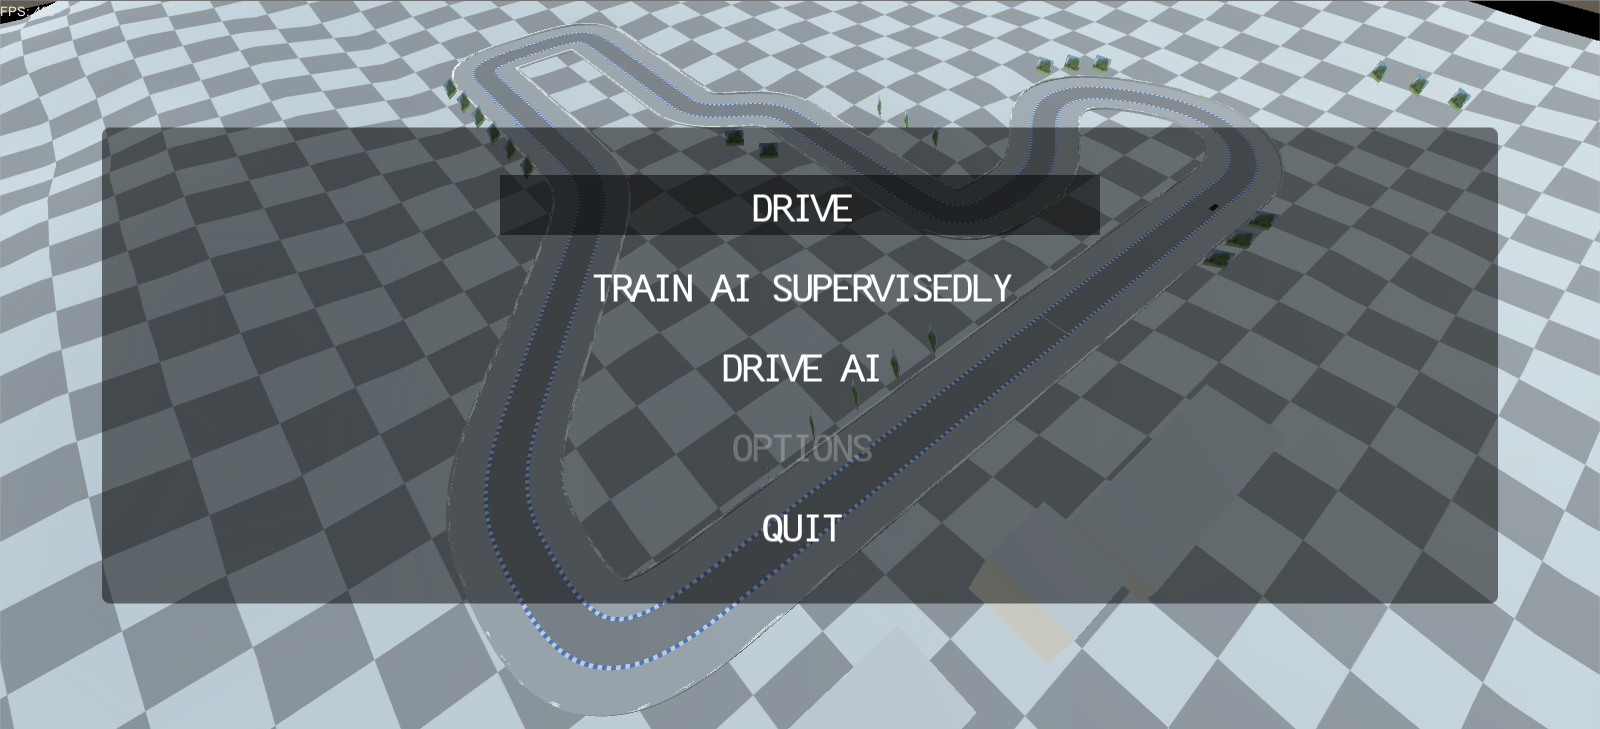
\includegraphics[width=\textwidth]{screenshot_overview}
	\centering
	\caption[Screenshot: menu of the game]{Start screen / menu of the game, also showing a bird-eye view of the track}
	\label{fig:overviewshot}
\end{figure}

\begin{figure}[h]
	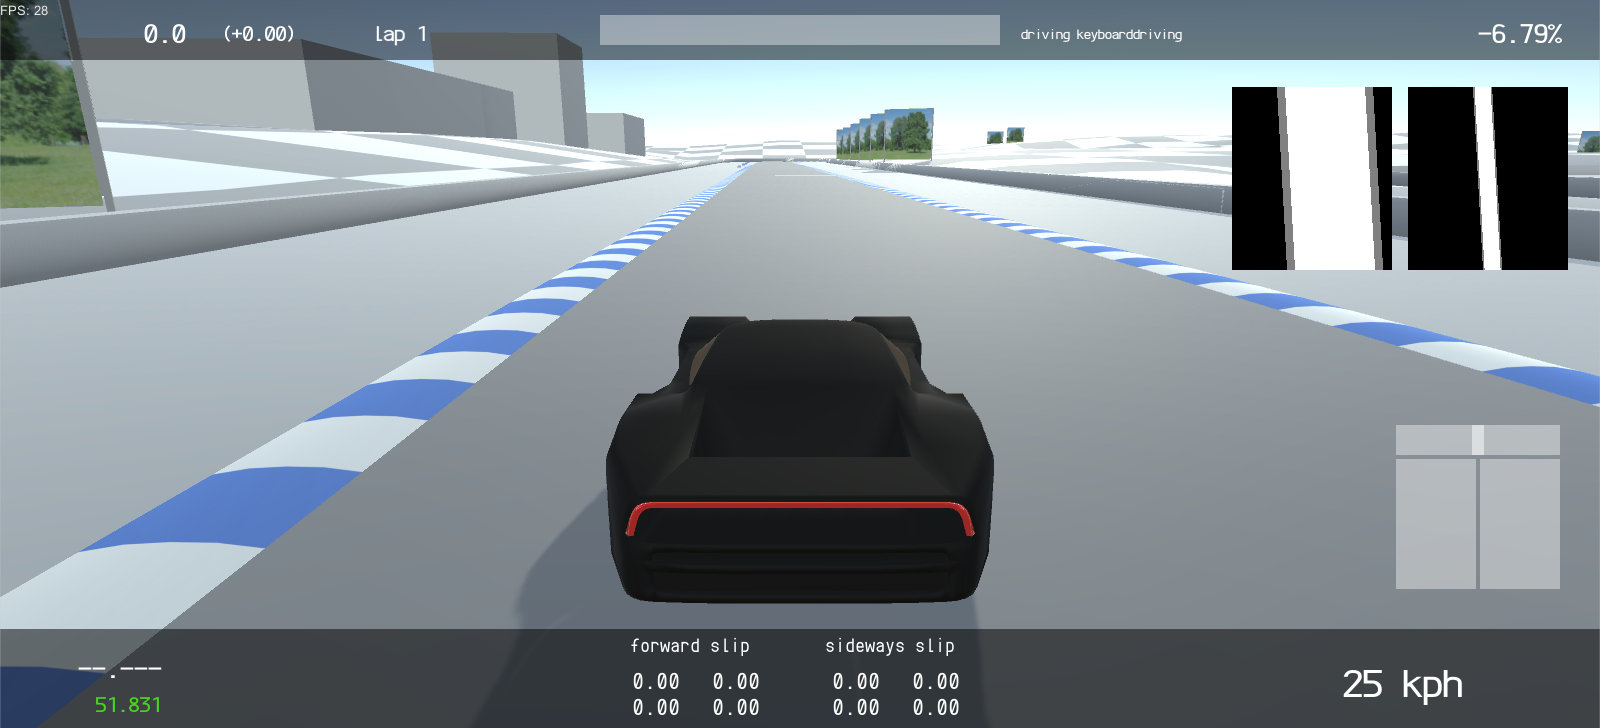
\includegraphics[width=\textwidth]{screenshot_human_juststarted}
	\centering
	\caption[Screenshot: Drive mode of the game]{\textbf{Drive} mode. For a description of the UI components, it is referred to section~\ref{ch:gamedescription}}
	\label{fig:humandriveshot}
\end{figure}

\begin{figure}[h!t]
	
	\centering
	\begin{annotatedFigure}
		{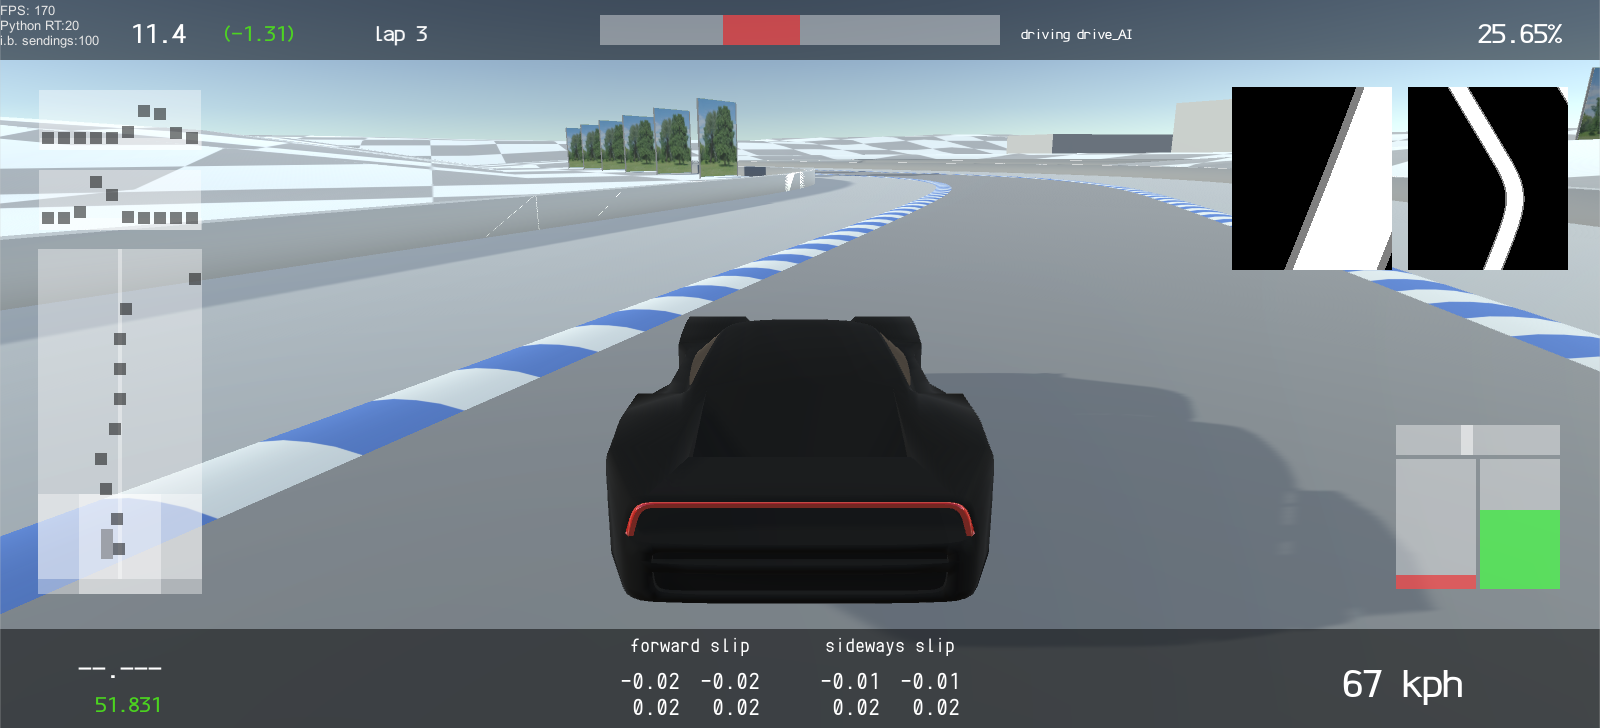
\includegraphics[width=\textwidth]{screenshot_driveAI}}
		\annotatedFigureBox{-0.002,0.9224}{0.0703,0.9951}{A}{0.0703,0.9224}%br
		\annotatedFigureBox{0.078,0.9208}{0.122,0.9813}{B}{0.122,0.9208}%br
		\annotatedFigureBox{0.1343,0.9223}{0.1946,0.9779}{C}{0.1946,0.9223}%br
		\annotatedFigureBox{0.224,0.926}{0.343,0.9769}{D}{0.343,0.926}%br
		\annotatedFigureBox{0.368,0.9295}{0.6303,0.99}{E}{0.6303,0.9295}%br
		\annotatedFigureBox{0.6363,0.9267}{0.8383,0.9823}{F}{0.8383,0.9267}%br
		\annotatedFigureBox{0.9043,0.9304}{0.989,0.9813}{G}{0.9043,0.9304}%bl
		\annotatedFigureBox{0.7663,0.6271}{0.8723,0.8937}{H}{0.7663,0.6271}%bl
		\annotatedFigureBox{0.8782,0.6231}{0.9843,0.89}{I}{0.9843,0.6231}%br
		\annotatedFigureBox{0.3743,0.1612}{0.6265,0.5963}{J}{0.6265,0.5963}%tr
		\annotatedFigureBox{0.0223,0.1963}{0.1283,0.6648}{N}{0.0223,0.1963}%bl
		\annotatedFigureBox{0.0243,0.7897}{0.1303,0.8849}{L}{0.1303,0.7897}%br
		\annotatedFigureBox{0.0222,0.6755}{0.1283,0.7713}{M}{0.1283,0.6755}%br
		\annotatedFigureBox{0.8683,0.1875}{0.981,0.4275}{K}{0.981,0.4275}%tr
		\annotatedFigureBox{0.0463,0.0073}{0.1083,0.0513}{Q}{0.1083,0.0513}%tr
		\annotatedFigureBox{0.0443,0.1656}{0.1063,0.3311}{O}{0.1063,0.1656}%br
		\annotatedFigureBox{0.3862,0.0029}{0.6083,0.1428}{R}{0.6083,0.1428}%tr
		\annotatedFigureBox{0.0443,0.0557}{0.1093,0.1153}{P}{0.1093,0.1153}%tr
		\annotatedFigureBox{0.8243,0.0293}{0.9283,0.0889}{S}{0.9283,0.0889}%tr
		\annotatedFigureBox{0.9623,0.0293}{0.9943,0.0908}{T}{0.9623,0.0908}%tl
	\end{annotatedFigure}
	
	\caption[Screenshot: Drive AI mode with annotations]{\textbf{Drive AI} mode, showing many additional information directly on the screen. For a description of those, it is referred to sections~\ref{ch:gamedescription} and \ref{ch:thevectors}}
	\label{fig:aidriveshot}
	\begin{itemize}
		\small
		\setlength\itemsep{0.1em}
		\item \textbf{A}: Debug information. Shows FPS, the agent's response time and the time in between two sendings to the agent (the latter two only visible in \term{drive\_AI} mode).
		\item \textbf{B}: The current lap time in seconds.
		\item \textbf{C}: The time difference of the current lap in comparison to the fastest lap so far.
		\item \textbf{D}: Indicator of the current lap. Also shows if a lap is \term{invalid}.
		\item \textbf{E}: Feedback bar, graphically visualizing the time difference of only the current course section in comparison to the fastest lap so far.
		\item \textbf{F}: Indicator for the current game mode. Also indicates if QuickPause is active or if a human interferes in the \term{drive\_AI} mode.
		\item \textbf{G}: Current track progress in percent.
		\item \textbf{H}: Field of view of the first minimap-camera.
		\item \textbf{I}: Field of view of the second minimap-camera, if enabled.
		\item \textbf{J}: The car. As the main camera is fixed behind it, it will always be in this precise position.
		\item \textbf{K}: Visual representation of the values for steering (top), brake-pedal (bottom left) and throttle pedal (bottom right).
		\item \textbf{L}: Visual representation of the game's \textit{progress-vector}. Only visible in \term{drive\_AI} and \term{train\_AI}.
		\item \textbf{M}: Visual representation of the game's \textit{CenterDist-vector}. Only visible in \term{drive\_AI} and \term{train\_AI}.
		\item \textbf{N}: Visual representation of the game's \textit{lookahead-vector}. Only visible in \term{drive\_AI} and \term{train\_AI}.
		\item \textbf{O}: Alternative representation of car's distance to the lane center. Only visible in \term{drive\_AI} and \term{train\_AI}. Overlapping with N due to low screen resolution on the machine used for the screenshot.
		\item \textbf{P}: Time needed for the last valid lap in seconds.
		\item \textbf{Q}: Time needed for the fastest valid lap (throughout different sessions) in seconds.
		\item \textbf{R}: Information about slip-behavious of the car's tires.
		\item \textbf{S}: Speed of the car in kilometers per hour.
		\item \textbf{T}: Indicates a "P" if the car is in reverse gear.
	\end{itemize}
\end{figure}
%TODO diese texte schöner, und for allem progress, centerdist und lookeahead einheitlich (nicht inlinecode? groß/klein genau wie imtext??)

\clearpage
\section{Agent}


\begin{figure}[h]
	{%
		\setlength{\fboxsep}{0pt}%
		\setlength{\fboxrule}{1pt}%
		\fbox{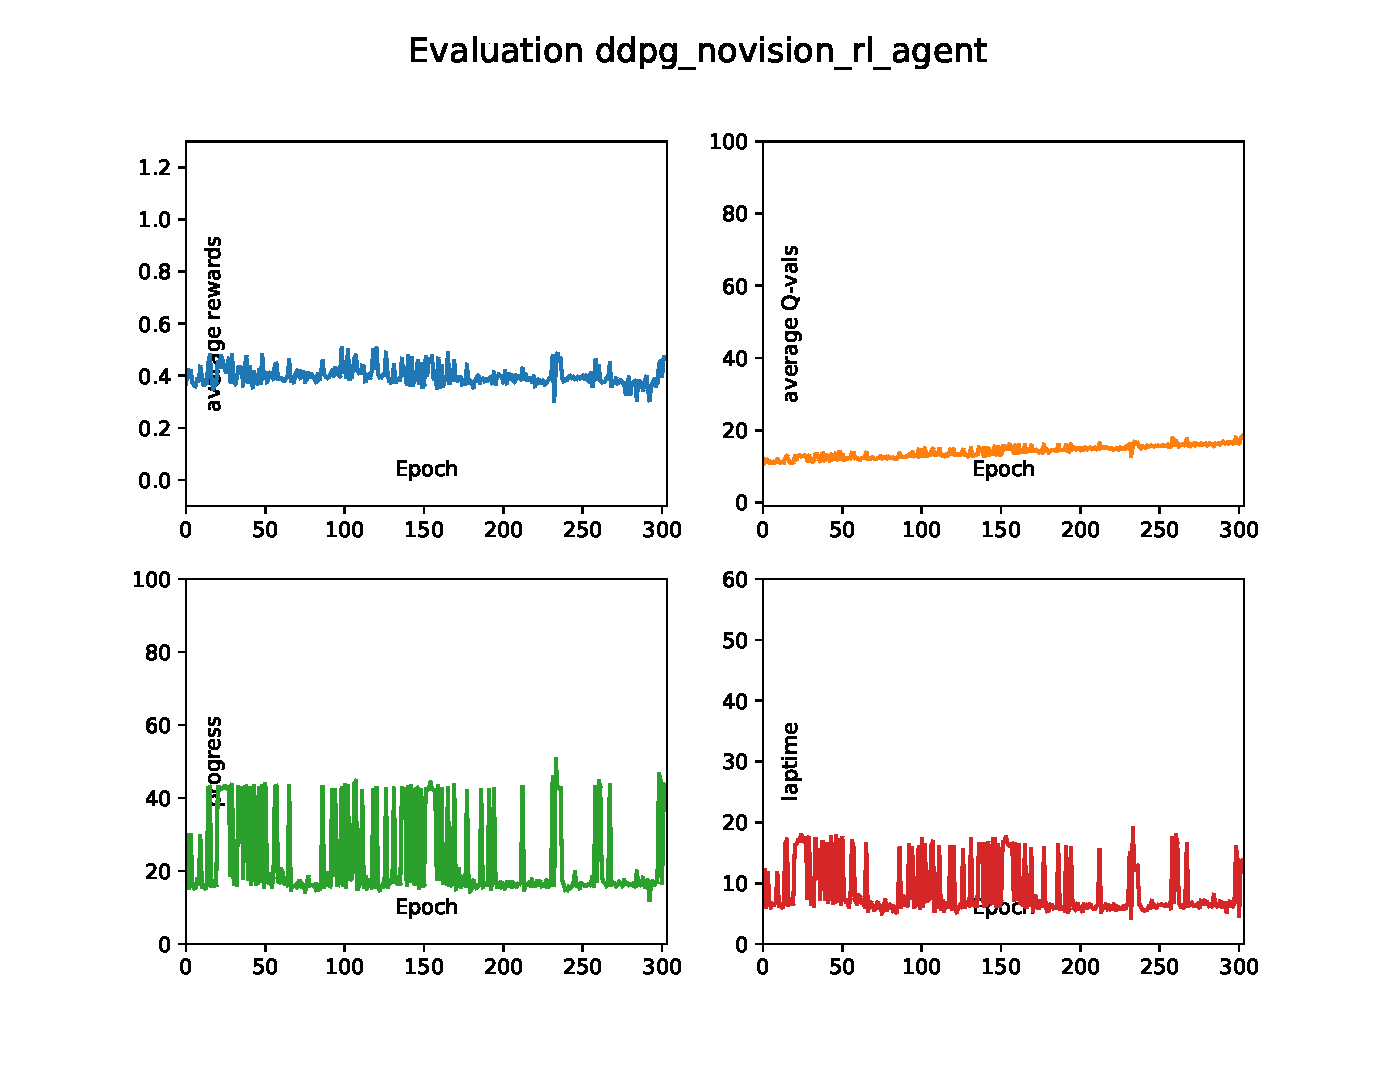
\includegraphics[width=.8\textwidth]{plot_figure}}%
	}%
	\centering
	\caption{A plot as the agent continually shows and updates during runtime}
	\label{fig:plot}
\end{figure}

\begin{figure}[h]
	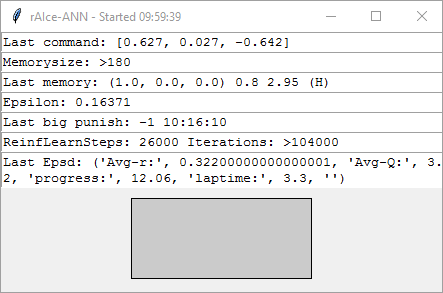
\includegraphics[width=.6\textwidth]{gui_shot}
	\centering
	\caption[Screenshot of the GUI in a typical run.]{Screenshot of the GUI in a typical run. The colored area at the bottom encodes the current reward via its intensity.}
	\label{fig:gui}
\end{figure}



\clearpage
\section{Vectors}

\begin{figure}[h]
	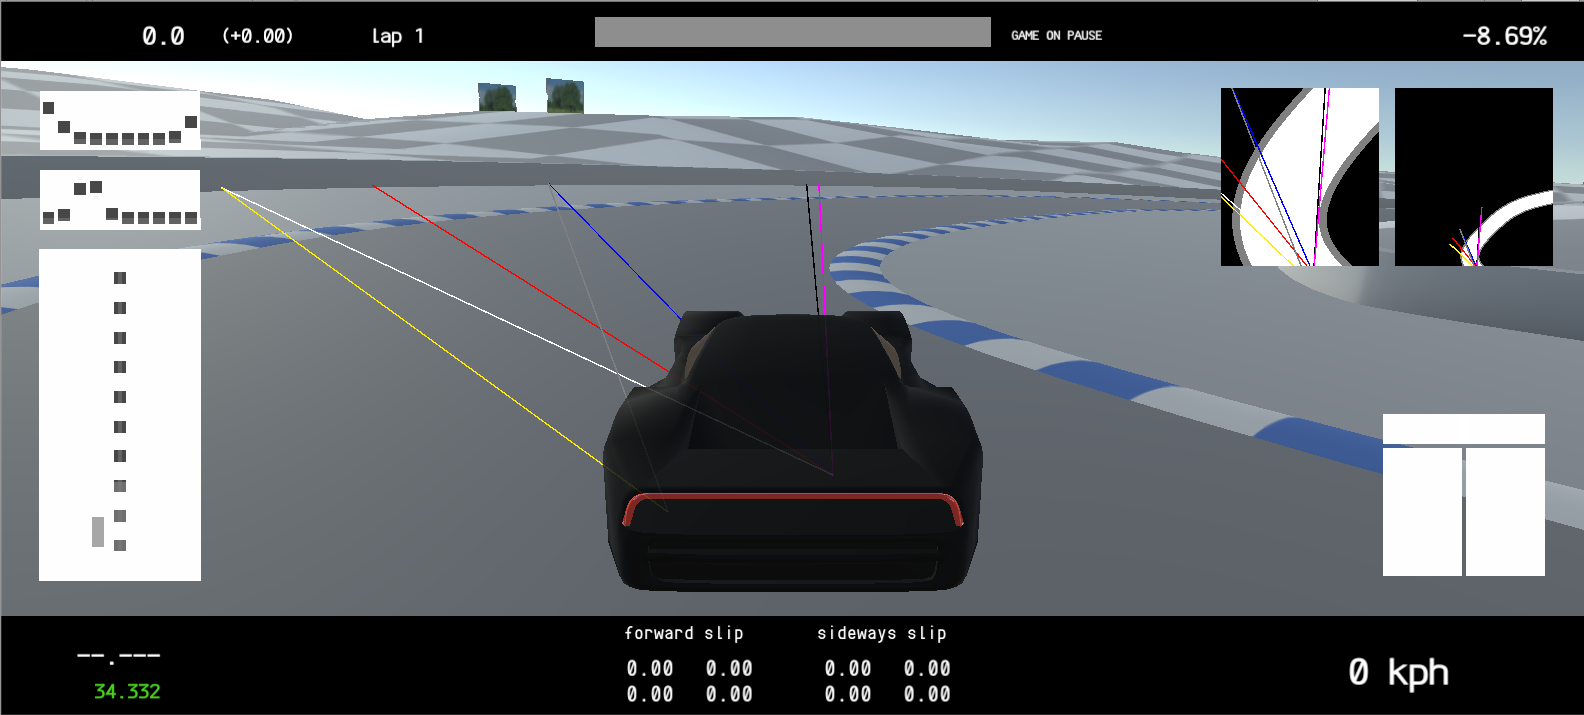
\includegraphics[width=\textwidth]{walldistvec}
	\centering
	\caption[Graphical representation of the rays used for the \term{WallDistVec}]{Graphical representation of the rays whose lenghts correspond to the \term{WallDistVec}. Note that the white and yellow ray as well as the blue and grey ray are actually parallel, as can be seen in the orthogonal minimap-cameras. To see these rays, \term{Gizmos} must be turned on in Unity.}
	\label{fig:walldistvec}
\end{figure}
	\restoregeometry
	%%% Appendix C
%
%
%\chapter{Complete UML-Diagrams of agents}
%
%
%\label{AppendixC}
%
%
%\begin{figure}[h!]
%	\centering 
%	\includegraphics[width=\textwidth]{uml_diagrams/agent_inText.2}  
%	\caption[UML-diagram of an agent and its super-classes]{incomplete UML-diagram of an agent and its super-classes. A more complete version can be seen in \colorbox{red}{appendix~\ref{BLABLABLA}}}
%	%\label{fig:agentMINI} 
%\end{figure}



		

	%----------------------------------------------------------------------------------------
	%	BIBLIOGRAPHY
	%----------------------------------------------------------------------------------------
	
	
	\printbibliography[heading=bibintoc]
	
	%----------------------------------------------------------------------------------------
	%	DECLARATION PAGE
	%----------------------------------------------------------------------------------------
	
	\begin{declaration}
		\addchaptertocentry{\authorshipname} % Add the declaration to the table of contents
		\noindent I, \authorname, hereby certify that the work presented here is, to the best of my knowledge and belief, original and the result of my own investigations, except as acknowledged, and has not been submitted, either in part or whole, for a degree at this or any other university.\\
		
		\vspace{10px}
		\noindent \rule[-0.3em]{25em}{0.5pt}\\ % This prints a line for the signature
		signature\\
		
		\vspace{4px}
		\noindent \rule[-0.3em]{25em}{0.5pt}\\ % This prints a line to write the date		
		city, date
		
%		\noindent I, \authorname, declare that this thesis titled, \enquote{\ttitle} and the work presented in it are my own. I confirm that:
%		
%		\begin{itemize} 
%			\item This work was done wholly or mainly while in candidature for a research degree at this University.
%			\item Where any part of this thesis has previously been submitted for a degree or any other qualification at this University or any other institution, this has been clearly stated.
%			\item Where I have consulted the published work of others, this is always clearly attributed.
%			\item Where I have quoted from the work of others, the source is always given. With the exception of such quotations, this thesis is entirely my own work.
%			\item I have acknowledged all main sources of help.
%			\item Where the thesis is based on work done by myself jointly with others, I have made clear exactly what was done by others and what I have contributed myself.\\
%		\end{itemize}
%		

	\end{declaration}
	
	\cleardoublepage
	
	%----------------------------------------------------------------------------------------
	
\end{document}  
